\documentclass{article}
\usepackage[utf8]{inputenc}

\usepackage[paper=a4paper, includefoot, margin=1cm, bottom=1cm]{geometry}
%\geometry{showframe, showcrop}
\usepackage{setspace}
\setstretch{1.35} %change this

\usepackage[english]{babel}
\usepackage{csquotes}
%Disable this for printing
\PassOptionsToPackage{hyphens}{url}\usepackage{hyperref}
\usepackage{titling, caption, xcolor}
\usepackage[newfloat]{minted}
\definecolor{LightGray}{gray}{0.9}

\newenvironment{code}{\captionsetup{type=listing}}{}
\SetupFloatingEnvironment{listing}{name=Source Code}

\usepackage[toc, page]{appendix}

\usepackage[utf8]{inputenc}
\usepackage[toc]{glossaries}
\setglossarystyle{listgroup}
\makeglossaries
\usepackage{glosseryterms}

\usepackage{lipsum}
\usepackage{environ}
\usepackage{pdfpages}

%plots / graphics
\usepackage{graphicx}
\usepackage{wrapfig}
\usepackage{pgfplots}
\usepgfplotslibrary[groupplots]
\pgfplotsset{compat=newest}

%math
\usepackage{float}
\usepackage{amsmath, amssymb, xparse}
%biblatex
\usepackage[style=apa, backend=biber]{biblatex}
\addbibresource{bibliography.bib}


%Definitions
\expandafter\def\expandafter\quote\expandafter{\quote\setstretch{1}}
%\RenewEnviron{figure}{}% Toggle this to get better page count
\newcommand*\colvec[1]{\begin{pmatrix}#1\end{pmatrix}}
\newcommand*\colmatrix[1]{\begin{bmatrix}#1\end{bmatrix}}


\title{Generating images using Generative Adversarial Neural Networks}
\author{Simon Felix Seeger}
\date{\today}

\begin{document}
\begin{titlepage}
    \begin{center}
        \vspace*{4cm}
        \Huge
       \textbf{\MakeUppercase\thetitle}
       \vspace{2cm}

       \textbf{\theauthor}

       \vfill
            
       \vspace{0.8cm}
        \begin{figure}[!ht]
            \centering
            
\includegraphics[width=0.3\textwidth]{images/rupprechtLogo.png}
            \captionsetup{textformat=empty,labelformat=empty}
            \caption{Rupprecht Logo; Source: \url{https://www.rupprecht-gymnasium.de/}}
        \end{figure}
       
       
       \Large    
       Supervising Teacher: Tim Storck\\
       Rupprecht Gymnasium München\\
       Bavaria, Germany\\
       \thedate
       \vspace{0.5cm}
        
    \thispagestyle{empty}
    \setcounter{page}{0}
    \end{center}
\end{titlepage}

\newgeometry{includefoot, inner=2.5cm,outer=4cm,top=2.5cm, bottom=1cm}

\tableofcontents
\listoffigures
\newpage


\section{Introduction}
With DALL$\cdot$E2 being able to generate images of stunning quality \autocite{ramesh_hierarchical_2022}, AI (Artificial Intelligence) generated imagery has increased in popularity\footnote{Based on Google Trends \url{https://trends.google.de/}}.
This is why this Paper discusses multiple Generative Adversarial Neural Networks (GAN) architectures and explains a model generating faces. GANs are, compared to for example diffusion model, an easy way to generate images. 

\section{Definitions}

\begin{itemize}
    \item The $\times$ symbol represents n-Dimensional shapes. For example a two dimensional array with a shape of $8\times 8$ holds 64 elements.
    \item Although machine learning algorithms use n-Dimensional Tensors\footnote{\textbf{Tensor:} Matrix optimized for machine learning arithmetic} for all calculations and data storage, this paper will use vectors and matrices interchangeably for simplicity.
    \item Long indexes are symbolized using square brackets to make equations more readable; short indices are represented by subscripts
\end{itemize}


\section{Basic Neural Network Architecture}
A neural Networks consists of layers, each passing their output to the next layer until the last one, called the output layer, is reached. 

\subsection{Perceptron}
A Perceptron takes one or more inputs and returns a value between 0 and 1 based on those inputs. The connection between the input $x_i$ and the Perceptron holds a weight $w_i$, which assigns a priority or importance to the input. The Perceptron itself also holds a bias $b$. The bias enables the Perceptron to reach the threshold easier or harder.
To make calculating the values of the Perceptron easier, both the inputs and weights are represented by a vector containing the corresponding values. The vectors are called $x$ and $w$ accordingly. Both are of the same site $m$. Each Perceptron calculates the function seen in equation~\ref{eq:Perceptron} \autocite[Chapter \textit{Using neural nets to recognize handwritten digits - Perceptrons}]{Nielsen:NNDP}.
\begin{equation}
    z(x)=
    \begin{cases}
        0,  & \text{if } b+\sum_{i=0}^m w_i \cdot x_i \leq \textit{threshold}\\
        1,  & \text{if } b+\sum_{i=0}^m w_i \cdot x_i > \textit{threshold}
    \end{cases}
    \label{eq:Perceptron}
\end{equation}

\subsection{Neuron}
\begin{figure}
    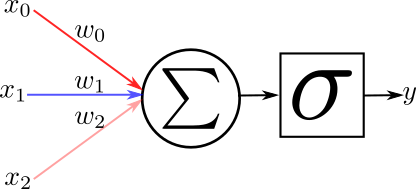
\includegraphics[width=0.33\textwidth]{images/Perceptron.png}
    \centering
  \caption{Example Structure Neuron}
  \label{fig:neuron}
\end{figure}
Neurons are modified Perceptrons. An example representation can be seen in figure~\ref{fig:neuron}. Here, the white circle is a Perceptron connected with the inputs $x$ using blue and red arrows. In this example the weights are represented, by the color. Red means that $w_i$ is a positive value, while a negative value has a blue connection. The stronger the color, the larger the value of $|w_i|$. 
Like the Perceptron, the neuron calculates the weighted sum as seen in equation~\ref{eq:neuron}.  In addition, the Neuron has an activation function $\sigma$
\begin{equation}
    y = \sigma\left(b+\sum_{i=0}^m w_i \cdot x_i\right)
    \label{eq:neuron}
\end{equation}

\subsection{Activation functions}
\label{ref:activation_functions}
The activation function of an layer is used to ensure that small changes to the weights and biases of a neuron don't affect the whole outcome in an unpredictable way \autocite[Chapter \textit{Using neural nets to recognize handwritten digits - Sigmoid Neurons}]{Nielsen:NNDP}. We will simplify this function as $\sigma(z)$. The parameter $z$ describes the ``raw'' output of the neuron. Commonly used functions can be seen in figure~\ref{fig:activation_functions}. 
Each of them serves an specific purpose depending on the type of model. The commonly used sigmoid neuron calculates: $$\frac{1}{1+e^{-\left(b+\sum_{i=1}^n w_i\cdot x_i\right)}}$$
\begin{figure}[H]
\centering
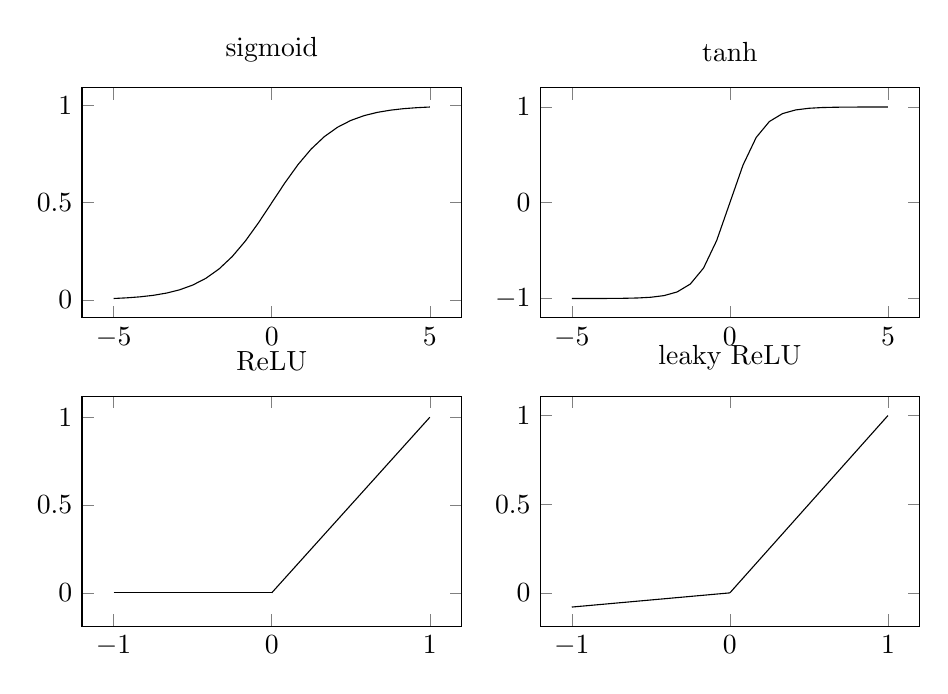
\begin{tikzpicture}
\begin{groupplot}[group style={
                   group name=activationFuncs,
                   group size= 2 by 2},height=4.5cm,width=6.4cm] 
\nextgroupplot[title=sigmoid]
    \addplot[] {1/(1+e^(-x))};
\nextgroupplot[title=tanh]   
    \addplot[] {tanh(x)};
\nextgroupplot[title=ReLU, ymin=-0.19]
    \addplot+[mark=none,black,domain=-1:0] {0};
	\addplot+[mark=none,black,domain=0:1] {x};
\nextgroupplot[title=leaky ReLU]
	\addplot+[mark=none,black,domain=-1:0] {0.08*x};
	\addplot+[mark=none,black,domain=0:1] {x};
\end{groupplot}
\end{tikzpicture}
\caption{Different activation functions commonly used in machine learning}
\label{fig:activation_functions}
\end{figure}
The other functions in this plot can be calculated as followed:\\
\textbf{tanh:} $$\sigma(x) = tanh(x)$$
\textbf{ReLU (Rectified Linear Unit):} $$\sigma(x) = 
\begin{cases}
    x, & \text{if } x > 0\\
    0, & \text{if } x \leq 0
\end{cases}$$
\textbf{leaky ReLU\footnote{usually $\alpha=0.01$}:} $$\sigma(x) = 
\begin{cases}
    x, & \text{if } x > 0\\
    \alpha x, & \text{if } x \leq 0
\end{cases}$$


\subsection{Loss function}
A loss function, also called error function, assigns a value to an output $\hat{y}$ of the model. This Value $Loss(\hat{y})$ depends on the expected output of the model. It is needed to optimize the model. The simplest of loss functions is the mean squared error seen in equation~\ref{eq:mean_squared_error}. 
\begin{equation}
    \label{eq:mean_squared_error}
    Loss(y) = (y-\hat{y})^2
\end{equation}
Let's take a model $M$ build to classify images into two categories: Cats ($y_{cat}=0$) and Dogs($y_{dog}=1$) as an example. If the model classifies a image of a cat with the value $\hat{y}=0.1$ then the loss of this image would be really small ($Loss(0.1)=0.01$) since $\hat{y}$ is close to the expected value. But if the model classifies the same image as a dog e.g $\hat{y}=1.8$, the loss increases ($Loss(1.8)=3.24$). The goal of a model is to minimize loss. 

\section{Common Machine Learning Terms}
\subsection{Convolutional layer}
\label{ref:conv_2d}
Convolutional layers enable finding detail across an image by calculating a part of the input with a filter $F$. The filter is often called the kernel. This process is called a discrete convolution. 
The trainable parameters are the values inside $F$ and the bias $b$. The \glspl{hyperparam} of a convolutional layer are the size and amount of filters, the stride (The amount of pixels the filter gets shifted each step) and the zero padding of the input image. \autocite{gu_recent_2017} 
In equation~\ref{eq:conv_2d} a function for two dimensional convolution using one filter of uneven size can be seen. Here $w_s$ and $h_s$ are the width and height of the strides and $w_F$ and $h_F$ the width and height of the filter respectively. Using this equation, the padding is dependent of the filter size and the index of the output image. 

\begin{equation}
    \label{eq:conv_2d}
    O[m,n] = I[m\cdot w_s-w_F:m\cdot w_s+w_F, n\cdot h_s-h_F:n\cdot h_s+h_F] \cdot F + b
\end{equation}
When the layer uses strides, the image is scaled down. Therefore the output size of a quadratic image can be calculated as followed with $o$, $i$ and $f$ being the size of the output image, input image and filter correspondingly.
\begin{equation}
    o = \frac{i+2p-f}{s}+1
\end{equation}
Convolutional layers proof as exceptionally useful in classification problems, where the object is not strictly centered but can be in any place of the image. Informal speaking a convolutional layer creates a map showing how much a part of an image represents the object.
\begin{figure}[!ht]
    \centering
    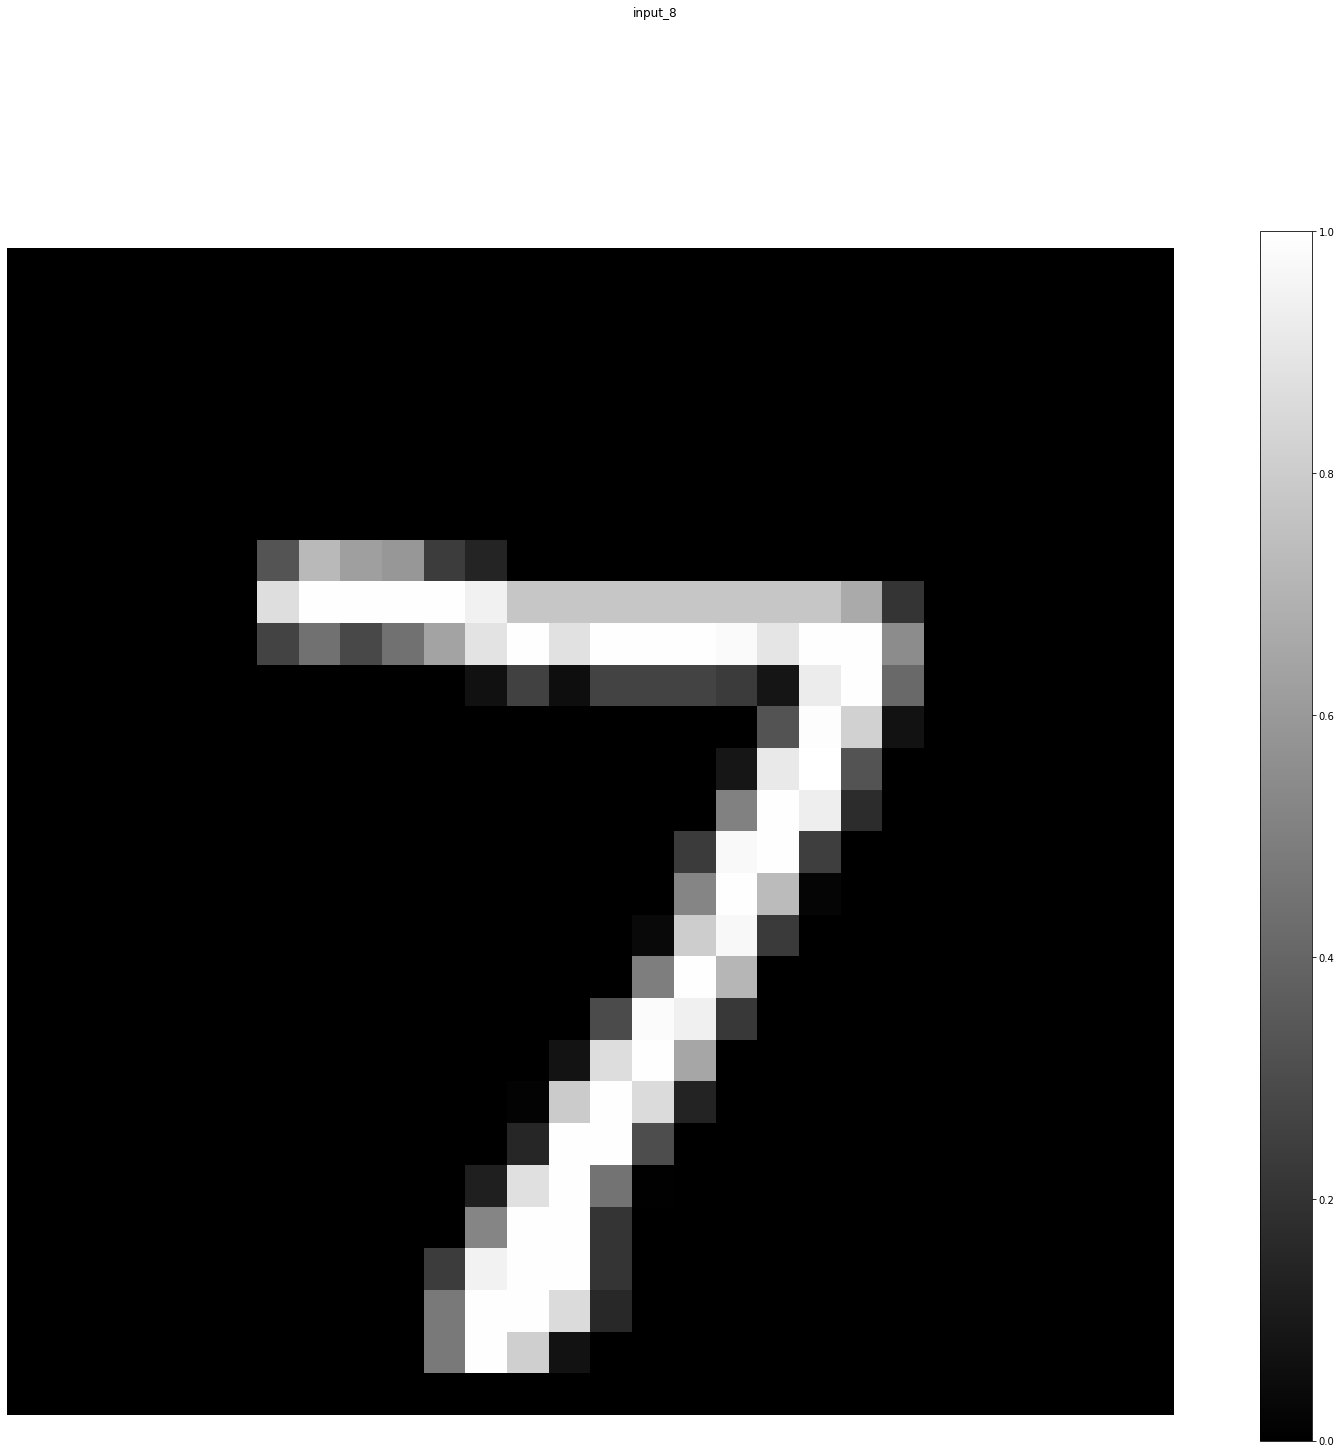
\includegraphics[width=.5\linewidth]{images/0_input_8.png}\hfill
    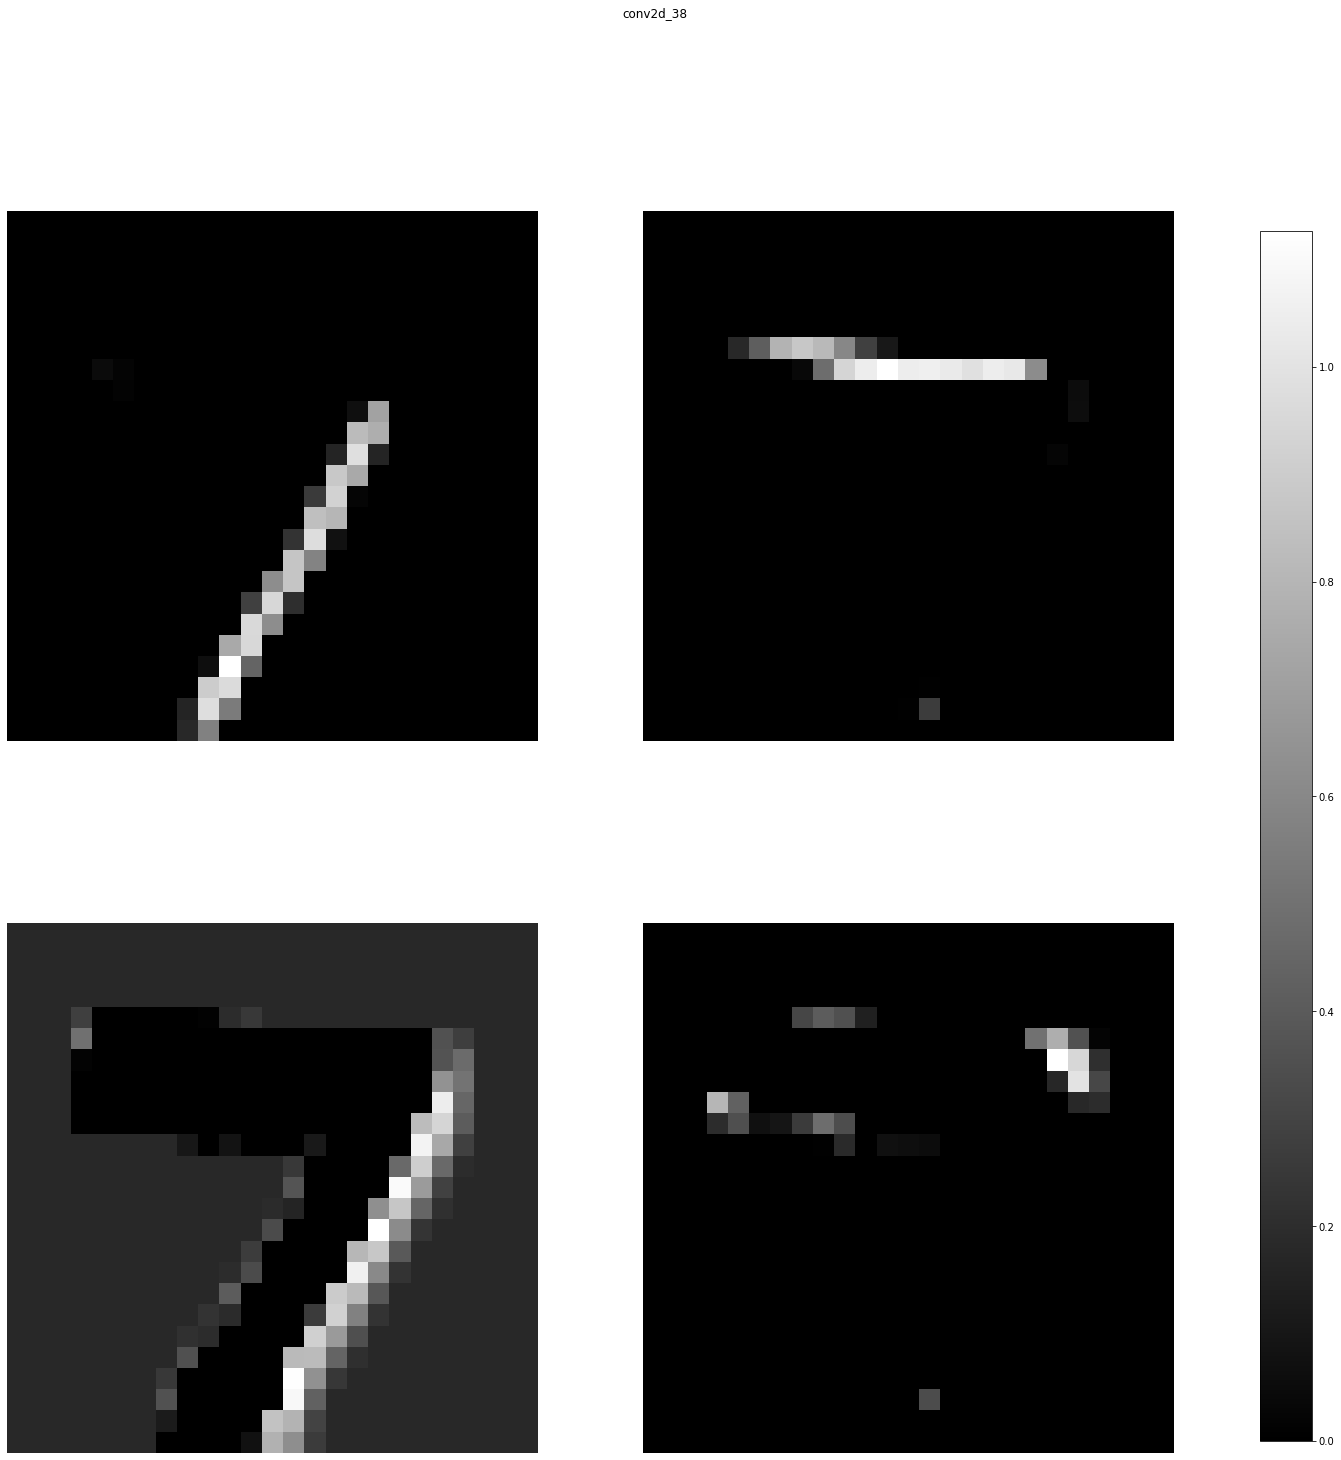
\includegraphics[width=.5\linewidth]{images/1_conv2d_38.png}\hfill
    \caption[Convolutional layer example]{\textbf{Left:} input image out of the MNIST Dataset \textbf{Right:} Feature maps after the first convolution}
    \label{fig:conv_feature_map}
\end{figure}
In image~\ref{fig:conv_feature_map} you can see an input image (left) out of the MNIST dataset\footnote{\url{http://yann.lecun.com/exdb/mnist/}}. On the right, you can see the feature maps generated by a filter. It is visible how the models filter pics up on key details of the number like the diagonal and top line of the seven. 

\subsection{Transpose layer}
\label{ref:transpose_2d}
While convolutional layers often reduce the size of the input matrix, transpose layers, also called deconvolution layers, increase the size of the input matrix using its filter $F$ when strided or padded. The resulting output size can be calculated like seen in equation~\ref{eq:transpose_size}
\begin{equation}
    \label{eq:transpose_size}
    o = (i-1)\cdot s + k - 2p
\end{equation}


\subsection{Binary Cross Entropy}
\label{ref:binary_crossentropy}
Binary Cross Entropy is a loss function commonly used for classification problems where data can be classified into a binary choice (e.g. yes or no). Given the label or expected value $y$ and the probability of a prediction, generated by the model, $p$, the loss can be calculated like seen in equation~\ref{eq:binary_crossentropy_single}. 
\begin{equation}
    \label{eq:binary_crossentropy_single}
    BCELoss(y, p) = -\left(y \cdot log(p)+(1-y)\cdot log(1-p)\right)
\end{equation}
When having multiple labels and predictions the loss can be calculated like seen in equation~\ref{eq:binary_crossentropy_cost}. $N$ in this case is the amount of labels.
\begin{equation}
    \label{eq:binary_crossentropy_cost}
    BCECost(y, p) = -\frac{1}{N}\sum^N_{i=1} y_i \cdot log(\hat{y_i})+(1-y_i)\cdot log(1-\hat{y_i})
\end{equation}
\begin{figure}[!ht]
    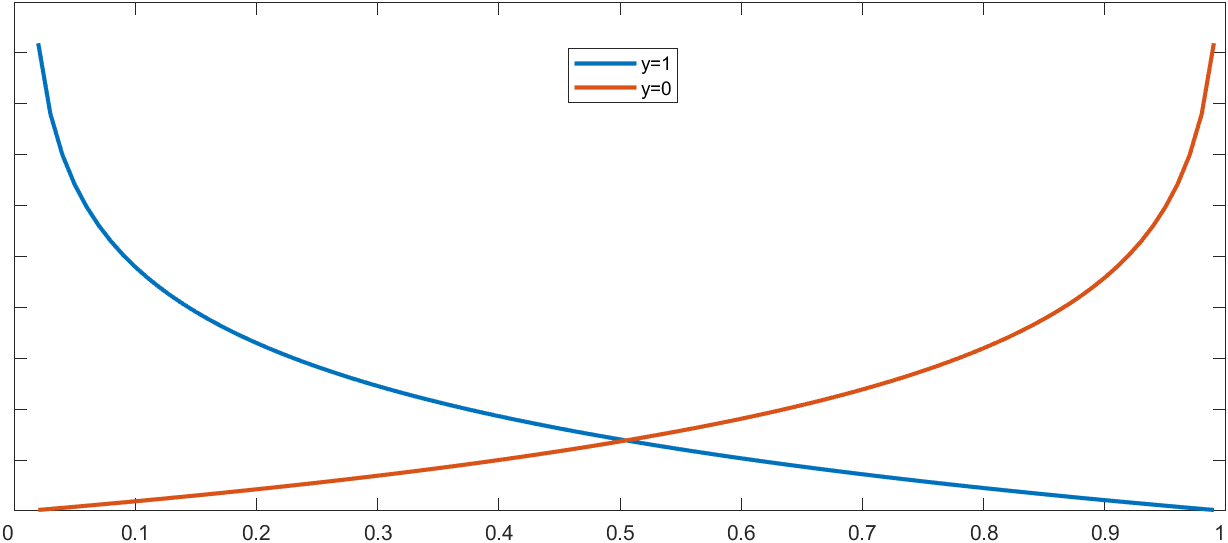
\includegraphics[scale=0.68]{images/logloss.png}
    \centering
    \caption{Binary Cross Entropy Loss}
    \label{fig:binary_crossentropy}
\end{figure}

The function~\ref{eq:binary_crossentropy_single} has some problems:\\
First, $\lim \limits_{x \to 1} Loss(1, x) = \infty$ and $\lim \limits_{x \to 0} Loss(0, x) = \infty$ meaning that $Loss(a, a); a\in \{0,1\}$ is undefined. A undefined loss means the model is unable to learn and adjust. Also, since the loss grows rapidly with values nearing the limit of the functions domain, optimizing the model gets uncontrollable. The easiest way to counter these effects is to clamp $p$ to a arbitrary range $[eps, -eps]$ with $0 < eps < 1$. The python package scikit-learn uses a value of $eps = 10^{-15}$.
Another problem is that models usually don't output probabilities, but logits, which are incompatible with the above defined loss function. To convert the floats into probabilities the sigmoid function can be used.\footnote{See \ref{ref:activation_functions} for more information on this particular activation function.} With $\sigma(x)=\frac{1}{1+e^{-x}}$ and $\hat{y}$ being the output of the model, the probability can be calculated as follows:
\begin{equation}
    p = \sigma(\hat{y})
\end{equation}
This updates the BCE Loss function to the one seen below.
\begin{equation}
    BCELoss(y, \hat{y}) = -\left(y \cdot log(\sigma(\hat{y}))+(1-y)\cdot log(1-\sigma(\hat{y})\right)
\end{equation}

\section{Preprocessing the training data}
To make the training of the models easier, the training data needs to be preprocessed. First of all, all images need to be scaled to the same size.
After resizing, the images have to be converted to tensors. The Tensor has the shape $w\times h\times 3$ with $w$ being the image width and $h$ the height. Since an \textit{RGB} image has three color channels, the tensor has a depth of 3. 
The last step is to clamp the color values of the image between -1 and 1 since Machine Learning Algorithms learn better with smaller numbers.


\section{Generative Adversarial Networks}
A Generative Adversarial Network (GAN) consists out of two models which are trained simultaneously: a Generator $G$ and a Discriminator $D$. While the Generator generates images, the Discriminator gets trained to differentiate between real images from the dataset and the images made by the Generator or simply put learns to distinguish real from fake images. $D$'s output is used to backpropate through $G$ and thus enables it's training process. The Generators goal is to deceive the Discriminator while $D$'s goal is to classify images perfectly.\\
All GANs need an input, for example a random vector of numbers to generate an output. The following subsections outline different kinds of GAN architectures, each with a different purpose or different advantages and disadvantages.

\subsection{Vanilla GAN}
\label{ref:vanilla_gan}
\begin{figure}[!ht]
    \centering
    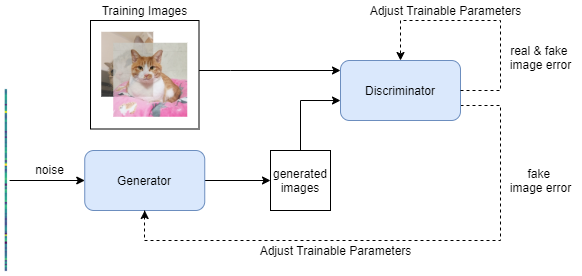
\includegraphics[scale=0.6]{images/DCGANBlackbox.png}
    \caption{Black box training diagram of a GAN; Cat Images from \url{https://www.microsoft.com/en-us/download/details.aspx?id=54765}}
    \label{fig:DCGANBlackbox}
\end{figure}
Vanilla GANs mostly use \glspl{dense} for both the Generator and Discriminator. Since \glspl{dense} are just matrix operations, this kind of GAN is the fastest out of all the following. 

\subsubsection{The Generator Model}
The Generator uses a latent vector $z$ containing normal distributed random values as its input. this vector gets passed through the network producing an image as the result. In a Vanilla GAN architecture, the network is composed of \glspl{dense}. 
Since the training data was normalized to values between -1 and 1, the tanh activation function is used for the Generators output.

The first \glspl{dense} has $w_I\cdot h_i \cdot n$ Neurons with $w_I, h_I, n \in \mathbb N _{\ne 0} \cap w_I < w_O, h_I < h_O$.\footnote{$w_0$ and $h_O$ being the size of the Output} $n$ is an arbitrary number. Continuing this process, the output of the previous layer is computed sequentially with multiple fully connected hidden layers, until the desired output shape is reached. 

\subsubsection{The Discriminator}
The Discriminator classifies images into how likely it is that the image is real. The closer this probability $p$ approaches 1, the more certain is the Discriminator that the image is out of the training set. The Discriminator is not able to output bigger probabilities than 1 since $p$ is a probability $1 \geq p \geq 0$ applies.

\subsubsection{Training the GAN}
\label{ref:GAN_training}
Since GAN training involves two models competing, a custom training loop is needed. In figure~\ref{fig:DCGANBlackbox} a black box training diagram for a GAN can be seen.\\
First noise needs to be generated which gets passed to the Generator. $G$ uses this latent vector the produce images $O_G$. The Discriminator evaluates $O_G$ and outputs a vector evaluating how real each image in the batch seems. We will call this $O_{D(G(z))}$.\\

While it is the Discriminators goal to maximize assigning the right values to images $x$, the Generator tries to minimize $\log(1-D(G(z))$. This minimax game between $G$ and $D$ gives this loss function the name Minimax Loss which was introduced in the paper by \citeauthor{goodfellow_generative_2014} \autocite*{goodfellow_generative_2014} and can be seen in equation~\ref{eq:minimax}. Here $E$ represents the expected value over all occurrences of real data or generated data. 
\begin{equation}
    \min\limits_G \max\limits_D V(D,G) =  E_{x}[\log(D(x))] + E_{z}[\log(1-D(G(z))]
    \label{eq:minimax}
\end{equation}
A problem with this function is, that the gradient in the early training process, in which $D$ has an easy job telling real and fake samples apart, is not sufficient to train the Generator. They propose letting $G$ maximize $\log(D(G(z))$ instead of minimizing $\log(1-D(G(z))$. This is the reason why $D$ uses the probability 1 for real images. 

Using equation~\ref{eq:minimax}, the gradients for the Discriminator can be calculated like seen in equation~\ref{eq:minimax_gradient_disc} with the batch size $m$ and the trainable parameters $\theta$.
\begin{equation}
    \label{eq:minimax_gradient_disc}
    \nabla_{\theta_d} \frac{1}{m} \sum^m_{i=0} \log(D(x_i)) + \log(1-D(G(z_i))
\end{equation}

In the same sense, the Generators gradients can be calculated visible in equation~\ref{eq:minimax_gradient_gen}
\begin{equation}
    \label{eq:minimax_gradient_gen}
    \nabla_{\theta_g} \frac{1}{m} \sum^m_{i=0} \log(1-D(G(z_i))
\end{equation}

%Since $G$ wants to fool $D$, the expected value is equal to 1, because this means the Discriminator classified generated images as real images. 
Because minimax loss is an alternation of the binary cross entropy loss, another way to rewrite it is using the $BCECost$ function. Therefore the Generators loss $Loss_G = BCECost(1, O_{D(G(z))})$. \\
In consideration of the Discriminator also having to learn the structure of real images, it is also shown a batch of real images, with the fake image batch and the real image batch being the same size. After producing the vector $O_{D(x)}$ for the real images, the Discriminator loss can be calculated as followed: $Loss_D = BCECost(0, O_{D(G(z))}) + BCECost(1, O_{D(x)}$.\\
It is important to note, that the Generator never sees real images, but only improves via $D$'s feedback.
%Since there is no way one can teach a machine how ``good'' an image looks, another way is needed to create a measurement for quality. 

\subsection{Deep Convolutional GAN}
\begin{figure}[!ht]
    \centering
    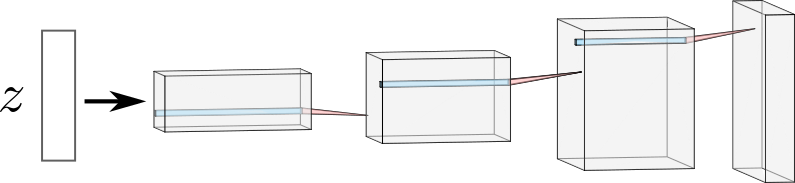
\includegraphics[width=0.5\linewidth]{images/DCGAN.png}
    \caption[AlexNet representation of a DCGAN's Generator; made with \url{https://alexlenail.me/NN-SVG/index.html}]{AlexNet representation of a DCGAN's Generator}
    \label{fig:dcgan_alexnet}
\end{figure}
Deep Convolutional GANs or DCGANs generate images using a convolutional architecture. The architecture was first introduced in a paper called \textit{Unsupervised Representation Learning With Deep Convolutional Generative Adversarial Networks} \autocite{radford_unsupervised_2016}.
Following this publication, there are some guidelines for building a DCGAN. First both $G$ and $D$ should use \gls{batchnorm}. Secondly the Architecture should follow the Convolutional Neural Network architecture specification. Third, the Adam optimizer should be used when possible and last, the Generator should use ReLu activation functions for all layers except the output which should be passed through the tanh function. The Discriminator should use leaky ReLU for all layers.
This means that the network uses transpose layers instead of \glspl{dense}. A example representation can be seen in figure~\ref{fig:dcgan_alexnet}

\subsubsection{The Generator}
The Generator of an DCGAN begins similar to a Vanilla GAN. The input layer has a shape of $n_z$, this gets passed down to a \gls{dense} with $w\cdot h\cdot n$ Neurons and a ReLU activation layer. The vector output of the \gls{dense} gets reshaped to a $h \times w\times n$ sized matrix. This way we can pass it into transpose layers until the desired Output shape $h_O\times w_O\times 3$ is reached. Each transpose layer has an ReLU activation function. More on transpose layers see section~\ref{ref:transpose_2d}. 

\subsubsection{The Discriminator Model}
The Discriminator has an input layer in the same shape as the training images. This image gets passed through multiple convolutional layers and gets flattened\footnote{Transforming the multi dimensional input into a vector Output} afterwards to enable processing the feature maps created by the Convolutional layers. The flattened vector is fed into a \gls{dense} with only one neuron. This is the output of the Discriminator. 

\subsection{Conditional GAN}
\begin{figure}[!ht]
    \centering
    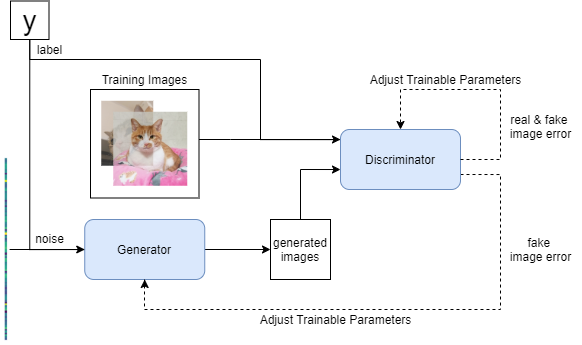
\includegraphics[scale=.6]{images/CGANBlackbox.png}
    \caption{Black box training diagram of a CGAN; Cat Images from \url{https://www.microsoft.com/en-us/download/details.aspx?id=54765}}
    \label{fig:CGAN_training}
\end{figure}
A conditional GAN or CGAN uses, in addition to the inputs described in section~\ref{ref:vanilla_gan}, labels provided through a secondary input in both Discriminator and Generator model. This architecture was introduced by \citeauthor{mirza_conditional_2014} \autocite*{mirza_conditional_2014}. They were able to generate for example numbers from the \textit{MNIST} dataset with the number generated resembling the label used while generating. Figure~\ref{fig:CGAN_training} shows a black box training diagram for CGANs.
\\
The updated objective function $V(D,G)$ for a CGAN can be seen in equation~\ref{eq:minimax_cgan}
\begin{equation}
    \label{eq:minimax_cgan}
    \min\limits_G \max\limits_D V(D,G) =  E_{x}[\log(D(x|y))] + E_{z}[\log(1-D(G(z|y))]
\end{equation}

\subsection{Problems}
\subsubsection{Mode Collapse}
\label{ref:mode_collapse}
\begin{figure}[!ht]
    \centering
    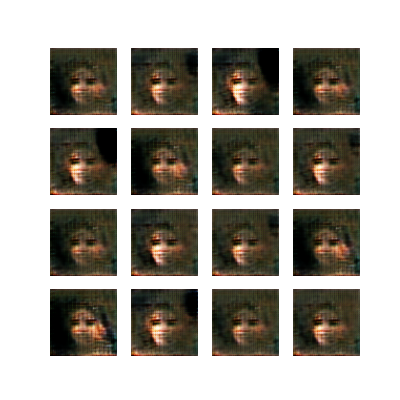
\includegraphics[width=.5\linewidth, trim={1.1cm, 1.1cm, 1.1cm, 1.1cm},clip]{images/image_at_epoch_0071.png}
    \caption{Output of an collapsed model}
    \label{fig:model_collapse}
\end{figure}
Mode collapse means that the Generator produces only similar looking images instead of the wanted variety and was already mentioned in the paper introducing Generative Adversarial Networks \autocite{goodfellow_generative_2014}. This is the case when $G$ finds a output which is particularly good at fooling the Discriminator and thus learns to only produce one kind of image. Since $D$ learns from generated images, it will reject all outputs generated by $G$. By doing so, the Discriminator gets stuck in a local minima leading to the Generator learning to generate a different set of homogeneous outputs. It is not possible to recover from mode collapse, since $G$ will always outplay the Discriminator by ``hopping'' from one local minima to another. \\
In figure~\ref{fig:model_collapse} mode collapse can be seen. Although there is some variety, many images look identical.

\subsubsection{Vanishing Gradients}
A vanishing gradient is a problem where while performing \gls{backpropagation} on deeper models, the gradient used is so insignificantly small, that it does not have any effect on the models performance or progress while training. Small gradients occur when the Discriminator gets too good at identifying the images made by the Generator and thus giving not enough information to train $G$. The vanishing gradient problem is not reserved to Generative Adversarial Networks but can happen in any deep neural network. While optimizing a model the derivatives of the layers get multiplied with each other layer after layer. With very small derivatives this leads to the gradient of the model in the end becoming extremely small and hence learning becomes nearly impossible. 

\subsubsection{Failure to converge}
When training a GAN, both the Generator and Discriminator compete against each other. This means, that a Generator performing exceptionally well makes the Discriminator less efficient and thus decreasing the value of the feedback generated by the Discriminator since $D$ comes close to randomly guessing if an image is generated or not. Especially on long training periods this can become an issue with the Generator starting to produce useless images to satisfy the improper advice.

\subsection{Improving image Quality}
\label{ref:image_quality}
\begin{wrapfigure}{l}{0.4\textwidth}
    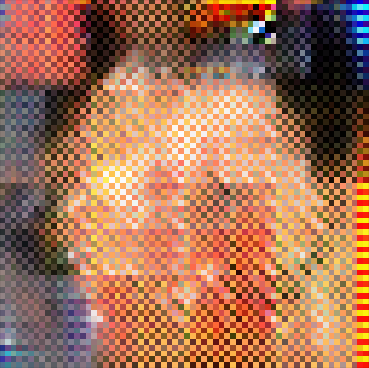
\includegraphics[width=.4\textwidth]{images/checkbord_image.png}
    \caption{Checkboard pattern created by uneven convolutions}
\end{wrapfigure}
One of the big problems while using transposed convolutions is the creation of checkboard pattern artifacts like seen in the image on the left. This is caused by uneven overlapping convolutions. ``In particular, deconvolution has uneven overlap when the kernel size [...] is not divisible by the stride [...]'' \autocite{odena2016deconvolution}.
In an ideal scenario, the model would learn to adjust to the checkboard pattern, but quite the opposite is true. It is even possible for models with even overlap to learn this kind of artifact \autocite{odena2016deconvolution}.\\
The article by \citeauthor{odena2016deconvolution} \autocite*{odena2016deconvolution} proposes resizing the images using a interpolation function and then using a convolutional layer to add detail to the image. This is process called ``resize-convolution''.

\section{Generating Faces using a Deep Convolutional Generative Adversarial Neural Network}
\label{ref:face_dcgan}
Artificial images of faces can be useful in many different applications. This includes copyright free images of people which can be used in advertising, media or anything where a face should represent a non existent person. A prime example of face generation is \url{https://thispersondoesnotexist.com/}. It uses the network SyleGAN2 introduced by \citeauthor{karras_analyzing_2020} \autocite*{karras_analyzing_2020}.\\
The approach I chose was building a DCGAN in python and training it on the CelebA\autocite{liu2015faceattributes} dataset which was not changed except a resize to $64\times 64$ pixels. 
\newpage
\subsection{Tensorflow Models}
Both models were created in the TensorFlow framework \autocite{tensorflow2015-whitepaper}. TensorFlow allowed me to create and experiment with the models in a quick manner. As described in Section~\ref{ref:vanilla_gan}, a generator and a discriminator model is needed. 

\subsubsection{The Generator Model}
\label{ref:faces_dcgan_gen}
The Generator uses a latent vector with the shape $n_z=128$ to provide enough input variance as input. The input layer is connected to a \gls{dense} with $4 \cdot 4 \cdot 256$ or $4096$ neurons and a ReLU activation function. To continue in a convolutional fashion, the vector outputted by the fully connected layer needs to be reshaped into a three dimensional matrix of shape $4\times 4\times 256$. The \gls{dropout} with a probability of 20\% prevents mode collapse, since the generator is not able to become too adjusted to the current iterations discriminator.
This layer is followed by 4 sets of transpose, leaky ReLU and batch normalisation layers. The transpose layers have a filter size of $2\times 2$, a stride of 2. 
The first Transpose layer or $n=0$ has 256, the second layer $n=1$ has 128 filter. Generally speaking the filter amount is determined by $\frac{256}{n\cdot 2}$
The output layer of the generator is a convolutional layer with a filter amount of 3, a filter size of $1\times 1$, a stride of 1 and the tanh activation function so that the Generator produces normalized image data. \\
The Generator plot can be seen in Figure~\ref{apx:dcgan_generator}.

\subsubsection{The Discriminator}
The Discriminator's input has the shape $64\times 64\times 3$, since this is the shape of the images in the dataset. Following this layer is a convolutional layer with 8 filters, each with a size of $3\times 3$ and no stride, an average \gls{pooling} layer and a leaky ReLU layer with $\alpha = 0.02$. These three layers get repeated three times, with the amount of filters increasing by a factor of 2. The first set of layers out of this collection has in addition a batch normalisation layer. The second has a additional \gls{dropout} with a dropout chance of 30\%. The last set has no additional layers but is followed by a flatten layer to convert the three dimensional matrix into a vector. The vector gets passed through a \gls{dropout} (30\% Dropout probability) into a \gls{dense} with 32 neurons followed by the output layer with one neuron.\\
A plot of the Discriminator can be seen in Figure~\ref{apx:dcgan_discriminator}.

\subsection{The training Loop}
\begin{minted}
[
frame=lines,
framesep=2mm,
baselinestretch=1.2,
bgcolor=LightGray,
fontsize=\footnotesize,
linenos
]
{python}
for i in range(self.d_steps):
    latent_vector = tf.random.normal(shape=(batch_size, self.latent_dim))
    with tf.GradientTape() as gt:
        generated_images = self.generator(latent_vector, training=True)
        prediction_fake = self.discriminator(generated_images, training=True)
        
        flipped_images = tf.image.random_flip_left_right(images)
        prediction_real = self.discriminator(flipped_images, training=True)
        
        d_loss = self.d_loss_fn(prediction_real, prediction_fake)
    d_gradients = gt.gradient(d_loss, self.discriminator.trainable_variables)
    self.d_optimizer.apply_gradients(zip(d_gradients, self.discriminator.trainable_variables))
\end{minted}
\captionof{listing}{Discriminator training loop}
\label{code:disc_train_loop}
The training loop was written using a class extending \texttt{keras.Model} and overwriting the \texttt{train\_step()} function so that I could use the \texttt{model.fit()} function and additional tools provided by TensorFlow like TensorBoard for measuring progress and callbacks to save images and checkpoints while training. \\
The discriminator training step can get repeated multiple times if needed. In the current version of the model, this is not needed, since the discriminator slowly converges. Each time a latent vector for the generator with the shape $batch\_size \times 128$ is generated using the \texttt{tf.random.normal()} function. This vector is passed into the generator producing a vector of images which are evaluated by the discriminator. To limit the change of the discriminator \gls{overfitting} and to introduce more variety, the training images get randomly flipped using the function \texttt{tf.image.random\_flip\_left\_right()} before being judged by $D$. The code for the discriminator training loop can be seen in Source Code~\ref{code:disc_train_loop}.
\\
The Generator train step is as describes in Section~\ref{ref:GAN_training}.\\
The loss is calculated as seen in Source Code~\ref{code:loss_functions}. It is important to note, that the binary crossentropy function has the \texttt{from\_logits} attribute set to true, so that the logits produced by the Discriminator can be used for cross entropy loss.\footnote{More on cross entropy loss can be read in Section~\ref{ref:binary_crossentropy}.} The function \texttt{discriminator\_loss(real\_output, fake\_output)} calculates $BCECost(1, O_{D(x)}) + BCECost(0, O_{D(G(z))})$. In the same code example it is also visible that the Adam optimizer with a learning rate of $1e-4$ is used for both $D$ and $G$. 

\begin{minted}
[
frame=lines,
framesep=2mm,
baselinestretch=1.2,
bgcolor=LightGray,
fontsize=\footnotesize,
linenos
]
{python}
cross_entropy = keras.losses.BinaryCrossentropy(from_logits=True)
def discriminator_loss(real_output, fake_output):
    real_loss = cross_entropy(tf.ones_like(real_output), real_output)
    fake_loss = cross_entropy(tf.zeros_like(fake_output), fake_output)
    total_loss = real_loss + fake_loss
    return total_loss

def generator_loss(fake_output):
    return cross_entropy(tf.ones_like(fake_output), fake_output)

generator_optimizer = tf.keras.optimizers.Adam(1e-4)
discriminator_optimizer = tf.keras.optimizers.Adam(1e-4)
\end{minted}
\captionof{listing}{custom loss functions for both $D$ and $G$}
\label{code:loss_functions}

\subsection{Problems while training}
Many training iterations failed due to mode collapse. To counter this I tried adding noise to the data passed into the Discriminator to decrease the chance of \gls{overfitting}. This however did not help as much increasing the length of the latent vector and removing some complexity from the generator.\\
Another problem was that the Discriminator learned too fast to distinguish the images and thus giving the Generator no meaningful feedback. Fortunately, since the loss of $D$ rapidly approaches zero, this issue can be identified early enough to avoid spending too much time training a model that is destined to fail. This time, reducing the filters by $\frac{1}{4}$ in all convolutional layers of $D$ resolved the problem. 

\subsection{Importing the Model into Matlab}
\begin{figure}
    \centering
    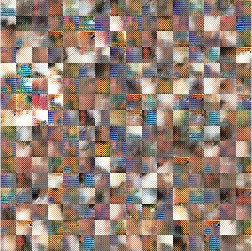
\includegraphics[width=0.5\textwidth]{images/rubbishImport_cropped.jpg}
    \caption{16 generated Images using imported model}
    \label{fig:rubbishImport}
\end{figure}
The model can be imported into Matlab by using the \texttt{importKerasLayers} function. It is important to also load the weights of the model, else model has to be trained again.\\
An additional step which has to be taken when using my generator is to replace the \texttt{tf.keras.layer.Reshape} layer with a custom function layer, since Matlab does have its own corresponding layer.
\begin{minted}
[
frame=lines,
framesep=2mm,
baselinestretch=1.2,
bgcolor=LightGray,
fontsize=\footnotesize,
linenos
]
{matlab}
layers = importKerasLayers("generator_model/generator.h5", "ImportWeights",true);

reshape_layer = functionLayer(@(x) dlarray(reshape(x, 4,4,256, []), "SSCB"), ...
                Formattable=true, Acceleratable=true);

layers_new = replaceLayer(layers, "reshape_1", reshape_layer);
generator = dlnetwork(layers_new);
\end{minted}
\captionof{listing}{Code to import the Generator}
\label{code:import_gen}
Although I was able to import the model, Matlab had problems interpreting the weights, giving me useless results like in figure~\ref{fig:rubbishImport}

\subsection{Results}
\begin{figure}[H]
    \centering
    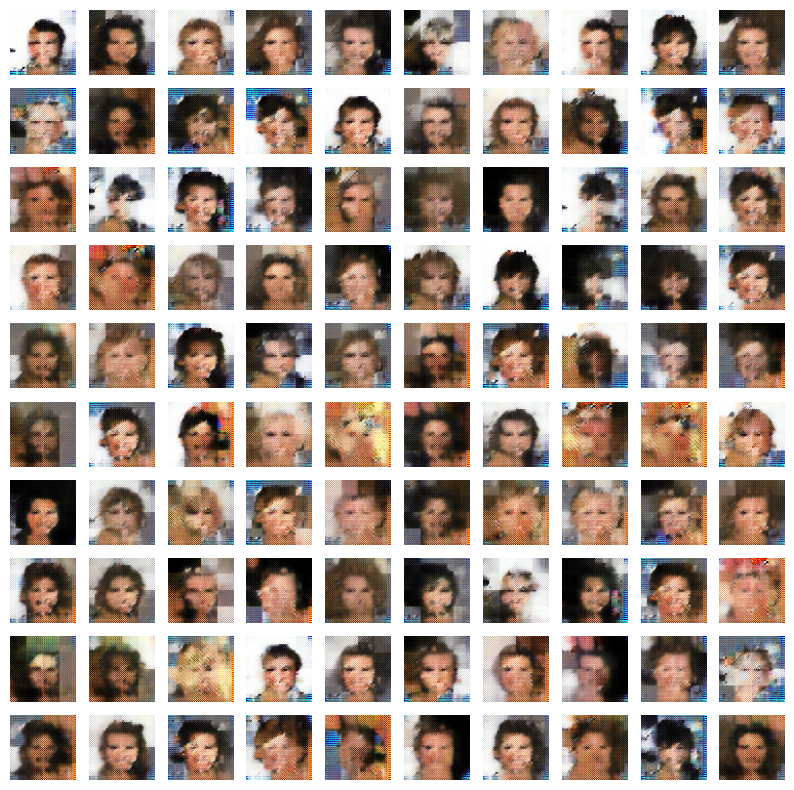
\includegraphics[width=0.7\textwidth]{images/faces.png}
    \caption{100 artificial faces}
    \label{fig:faces_dcgan}
\end{figure}
The images visible in figure~\ref{fig:faces_dcgan} were generated by the model described in section~\ref{ref:faces_dcgan_gen}. This Generator was trained for 455 Iterations. More Images can be generated using the script~\ref{apx:generation_code}.
This model has clearly some flaws. First of all, the image quality is not great. Some faces are not recognizable, others consist mostly out of black pixels. To improve this the generator network needs to be refined and more training epochs are needed. Second the images suffer from the check board pattern associated with transposed convolutions. More on how to prevent this effect can be read about in section~\ref{ref:image_quality}.\\
Implementing the aforementioned changes, the image quality could be greatly improved.\\
Additional Images generated during training can be found on the USB-Stick or at \url{https://github.com/SFSeeger/w-seminar}. The code is also available in the appendix: \ref{apx:celebGAN}.

\subsection{celebGAN2}
CelebGAN2 is a project which I made to improve image Quality of the first model. I was not planning on showing it, since it was training while writing this paper and not producing any results showing improvement. This changed however as soon as i saw this paper as completed. \\
This GAN was trained in 319 iterations. Both the generator and Discriminator Loss can be found in the appendix in section~\ref{apx:celebGAN2Loss}.
\subsubsection{Changes}
Changes were only done to the generator. These changes are moving the Batch normalisation layer before the leaky ReLU layer and changing the last convolution layer to use a kernel size of $4\times4$ and zero-padding. 
\subsubsection{Results}
\begin{figure}[H]
    \centering
    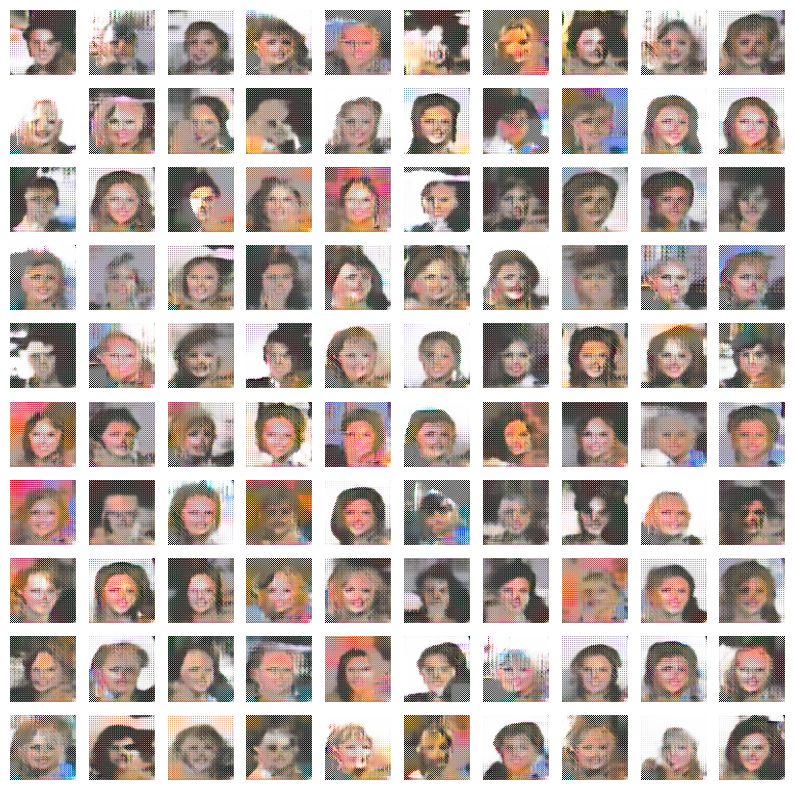
\includegraphics[width=0.7\textwidth]{images/faces2.png}
    \caption{100 Images of celebGAN2}
    \label{fig:pred_celebGAN2}
\end{figure}
The Results are visible in Figure~\ref{fig:pred_celebGAN2}. As shown the faces are better recognisable than in Figure~\ref{fig:faces_dcgan} which is promising. But this model still has some issues. First, the Images are less saturated and vibrant as the images produced by the first version of the model and the checkboard effect is still visible. In addition is the background stronger blurred. The code is available in the appendix: \ref{apx:celebGAN2}.

\section{Additional Experiments}
\subsection{conditional DCGAN}
I also tried building a conditional Deep convolutional Neural Network to generate faces\footnote{using the CelebA Dataset\autocite{liu2015faceattributes}} based on a label specifying the gender of the generated person. The code for it can be found in the file \textit{DCGAN.ipynb} or in the appendix: \ref{apx:DCGAN}. This model however suffered from mode collapse. The image seen in Section~\ref{ref:mode_collapse} was an output one of the many collapsed GANs produced and I was not able to make the model work reliably. An overhaul of the network architecture would be needed to resolve this issue. This would include changing the loss function to for example the Wasserstein loss \autocite{arjovsky_wasserstein_2017}. \\

\subsection{Matlab DCGAN}
This was an attempt to use Matlab's Deep Learning Toolbox to generate handwritten digits using the \texttt{digitTrain4DArrayData} Dataset. This attempt was unsuccessful, because the Generator did not converge. Here, a change in Discriminator architecture and the use of a better training loop could return satisfying results. The code can be found in the file \textit{GAN.mlx} or in the appendix: ~\ref{apx:MLGAN}

\section{Conclusion}
In conclusion, Generative Adversarial Neural Networks are reliable network that can generate digital images with good quality. However, this requires overcoming the instability of the network using various techniques.\\
With the models introduced in this paper (\textbf{celebGAN} and \textbf{celebGAN2}) I was able to show some of what can be achieved using Generative Adversarial Neural Networks. Although the images generated by both models suffered from artifacts, faces were recognisable, which shows that both models understood which attributes a face needs to be identifiable. \textbf{CelebaGAN2} was able to generate images of higher quality in fewer iterations. This can probably be attributed to the convolutional layer with a larger kernel. Unfortunately, due to lack of time, I was not able to make the other models and processes described in this paper functional. \\
A future goal I set myself is to improve the \textbf{celebGAN2} architecture to generate images with higher quality. It is to be expected that AI generated imagery will play a greater role in our society by supporting the creative process in modern media like games, movies or advertising. 
All code referenced here and the images generated by the models detailed above can be found on the included USB-Stick or at \url{https://github.com/SFSeeger/w-seminar}.

\clearpage\printbibliography
\clearpage\printglossary[toctitle=Glossary]

\begin{appendix}
\clearpage
\section{Additional Content for Section~\ref{ref:face_dcgan}}
\subsection{Generator Plot}
\label{apx:dcgan_generator}
\begin{figure}[H]
    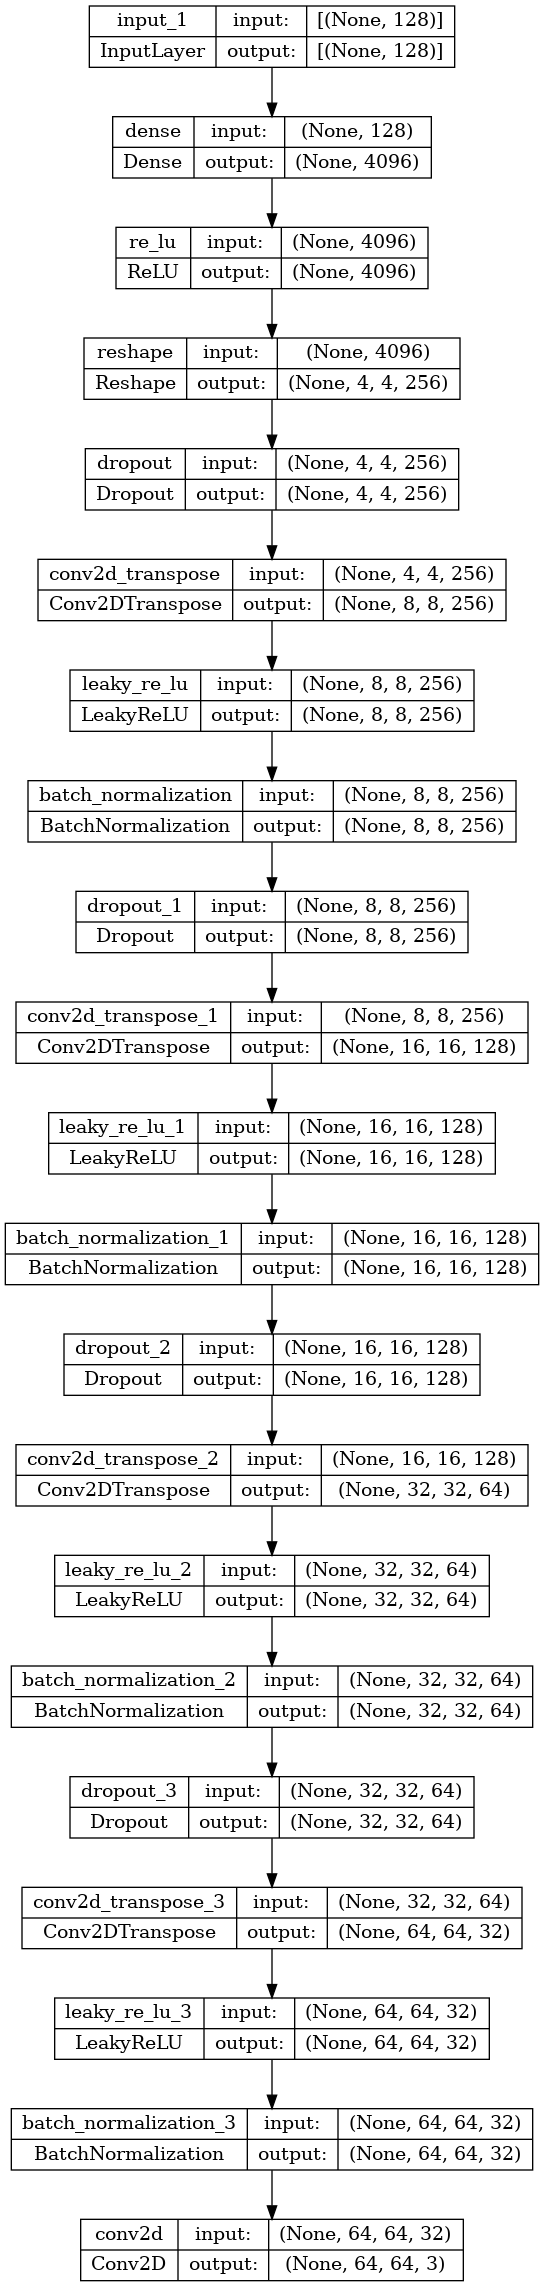
\includegraphics[width=.36\textwidth]{images/Generator.png}
    \centering
    \caption{Generator used for celebGAN}
\end{figure}

\subsection{Discriminator Plot}
\label{apx:dcgan_discriminator}
\begin{figure}[H]
    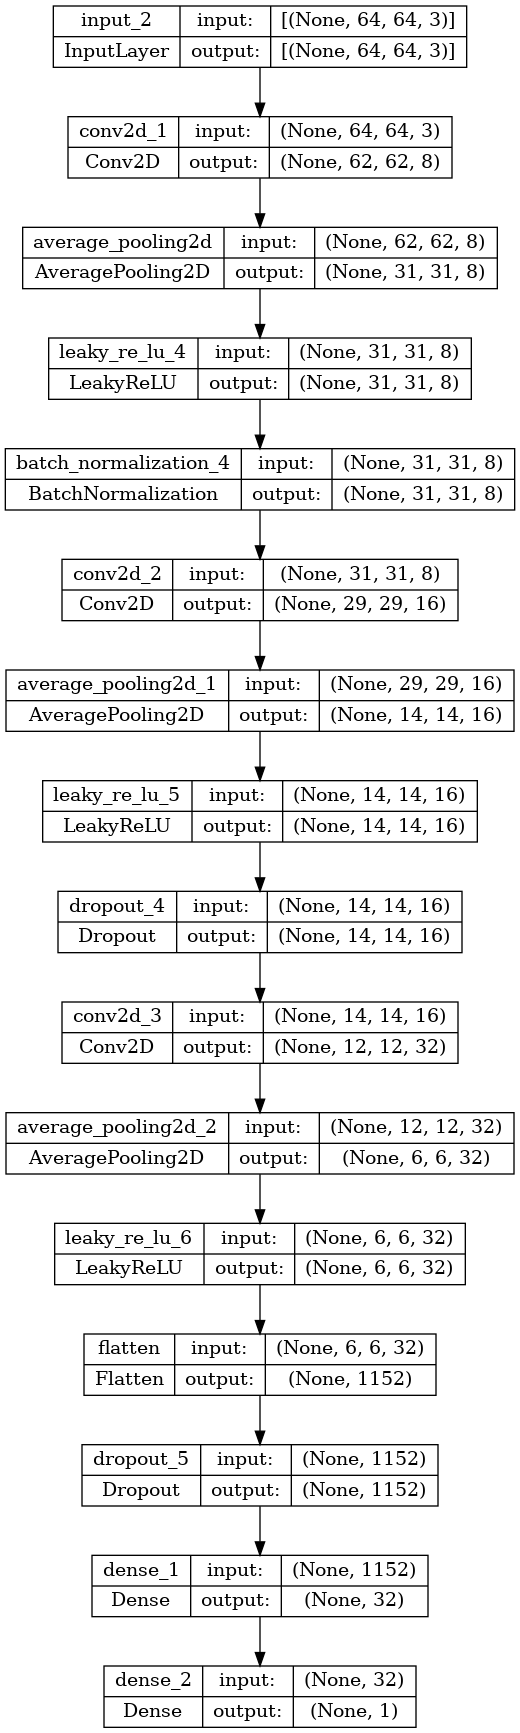
\includegraphics[width=.35\textwidth]{images/Discriminator.png}
    \centering
    \caption{Discriminator used for celebGAN}
\end{figure}

\subsection{Image Generation Code}
\label{apx:generation_code}
\begin{minted}
[
frame=lines,
framesep=2mm,
baselinestretch=1.2,
bgcolor=LightGray,
fontsize=\footnotesize,
linenos
]
{python}
import tensorflow as tf
import matplotlib.pyplot as plt
import numpy as np

generator = tf.keras.models.load_model('celebGAN/generator_model/generator.h5')

#for single image
lv = tf.random.normal([1, 128])
image = generator(lv)
imagenorm = image*127.5+127.5
imagenp = imagenorm.numpy()[0,:,:,:]
plt.imshow(imagenp.astype(dtype="int32"),
    interpolation='antialiased', interpolation_stage="rgba")

#for multiple images
images = 25
predictions = np.empty([100,64,64,3])
for i in range(4):
    seed = tf.random.normal([images, 128])
    label_seed = np.random.randint(0,2, images)
    pred = generator(seed, training=False).numpy()
    predictions[25*i:25*(i+1), :, :, :] = pred
    
print(predictions.shape)
figsize = 10
fig = plt.figure(figsize=(figsize, figsize))  
for i in range(predictions.shape[0]):
    plt.subplot(figsize, figsize, i+1)
    plt.imshow((predictions[i, :, :, :]*127.5+127.5).astype("int32"),
        interpolation='antialiased', interpolation_stage="rgba")
    plt.axis('off')
plt.show()
\end{minted}
\subsection{Loss for celebGAN2}
\label{apx:celebGAN2Loss}
\begin{figure}[H]
    \centering
    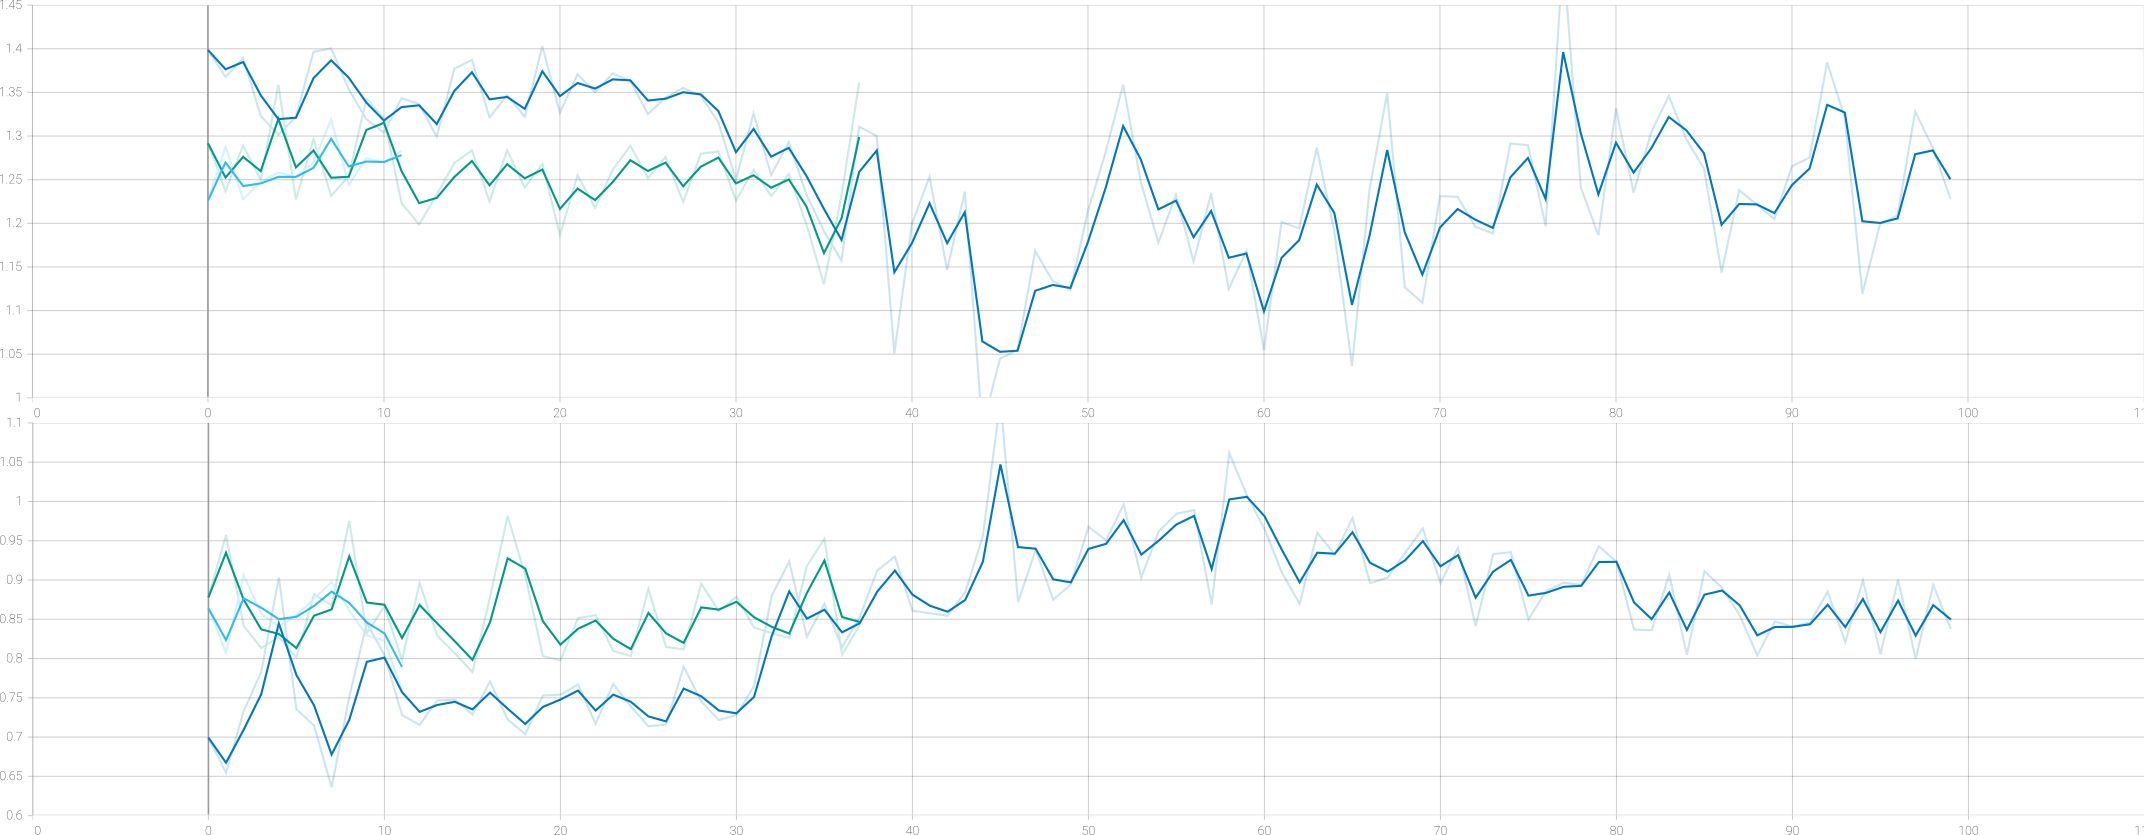
\includegraphics[width=0.9\textwidth]{images/BothLoss.png}
    \caption{\textbf{Top:} Discriminator Loss. \textbf{Bottom:} Generator Loss; Each line represents a training process at a different time}
    \label{fig:my_label}
\end{figure}

\section{Code}

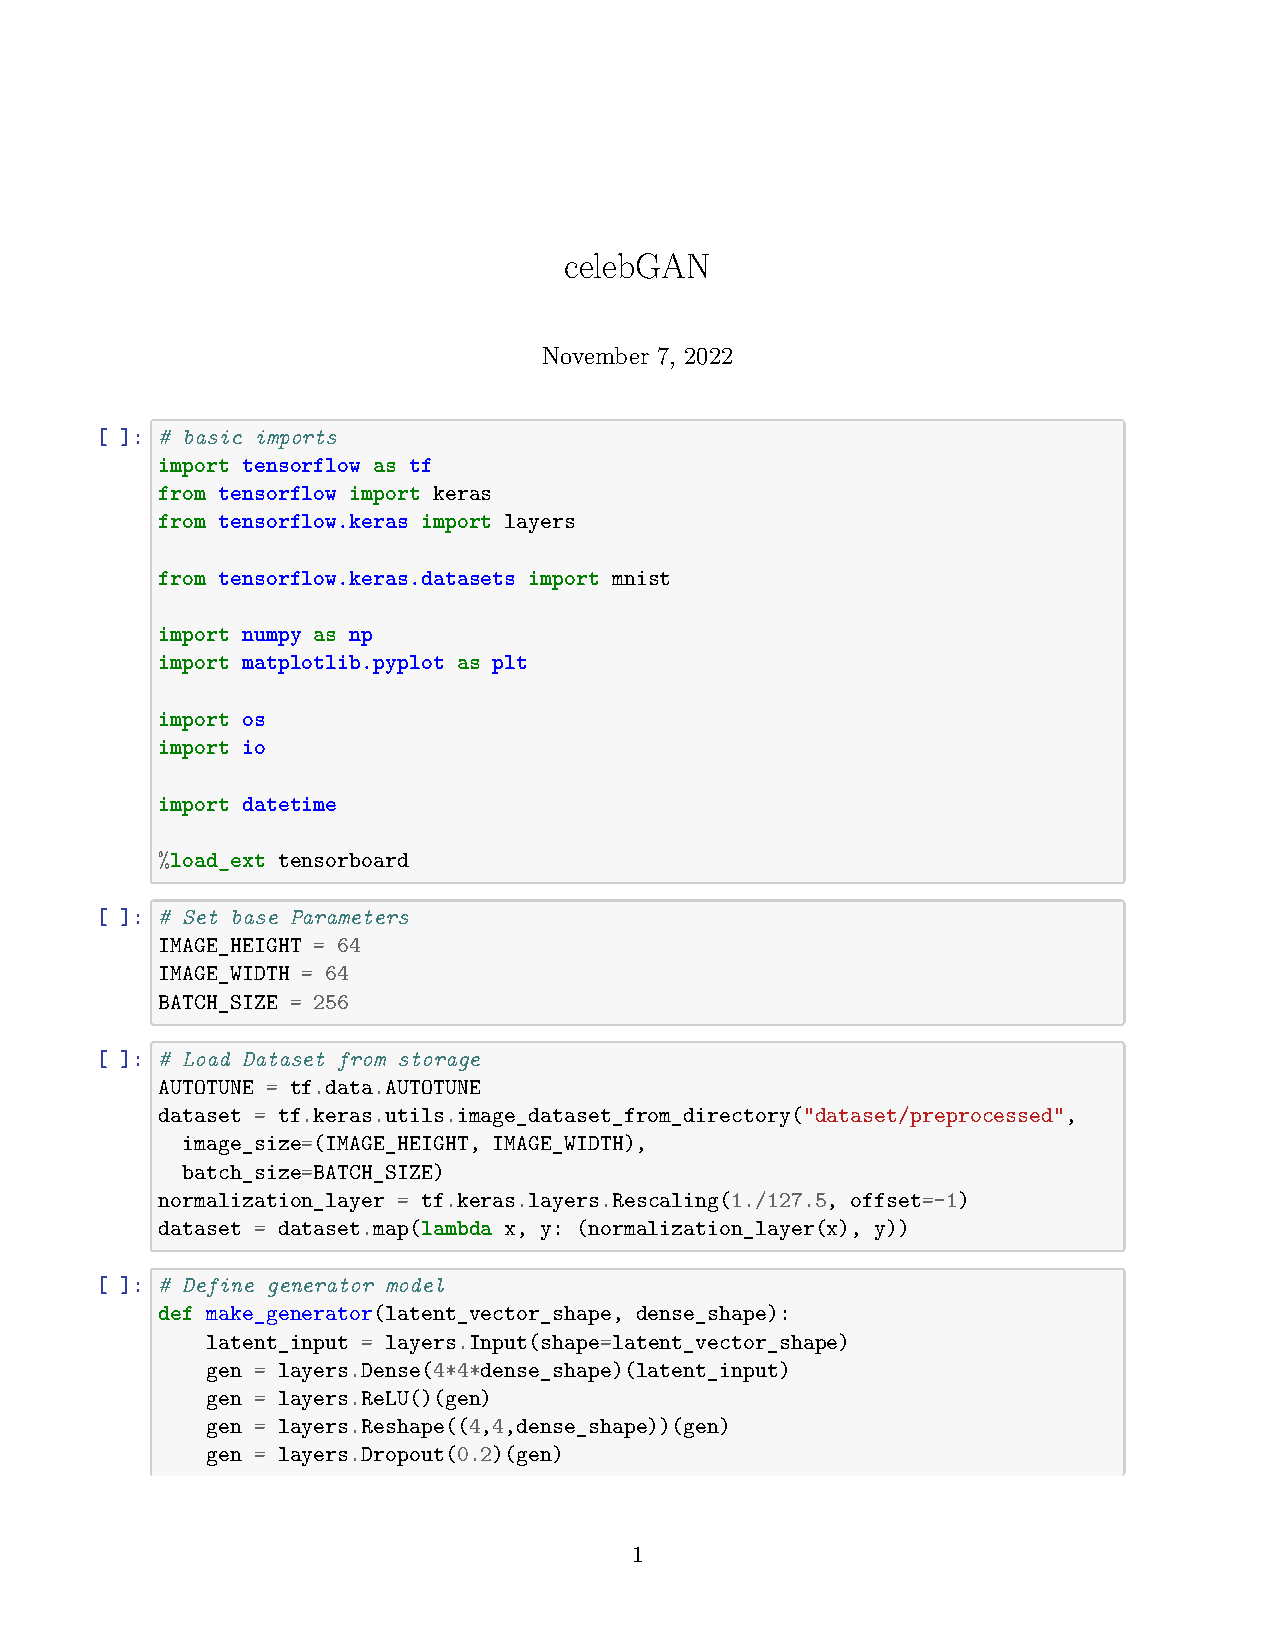
\includepdf[pages=-, addtotoc={1,subsection,2, celebGAN, apx:celebGAN}]{code/celebGAN.pdf}
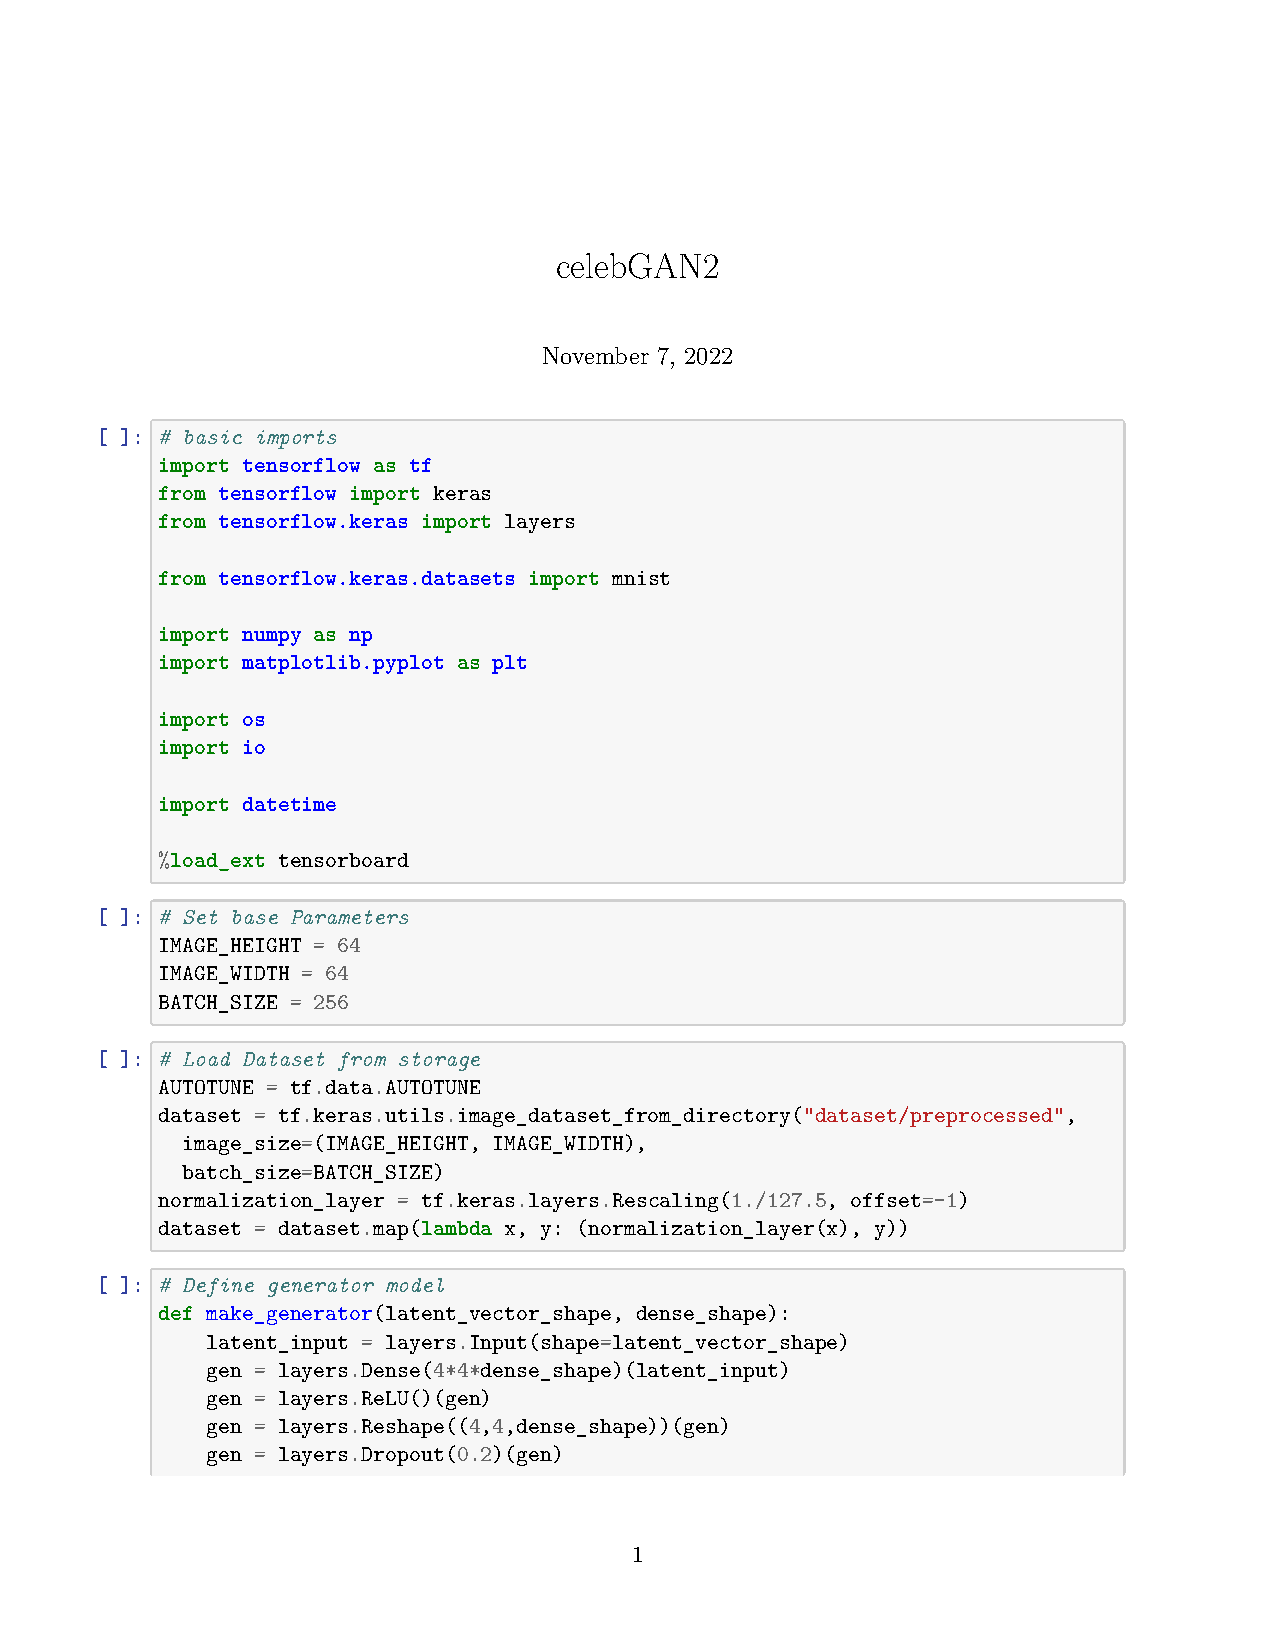
\includepdf[pages=-, addtotoc={1,subsection,2, celebGAN2, apx:celebGAN2}]{code/celebGAN2.pdf}
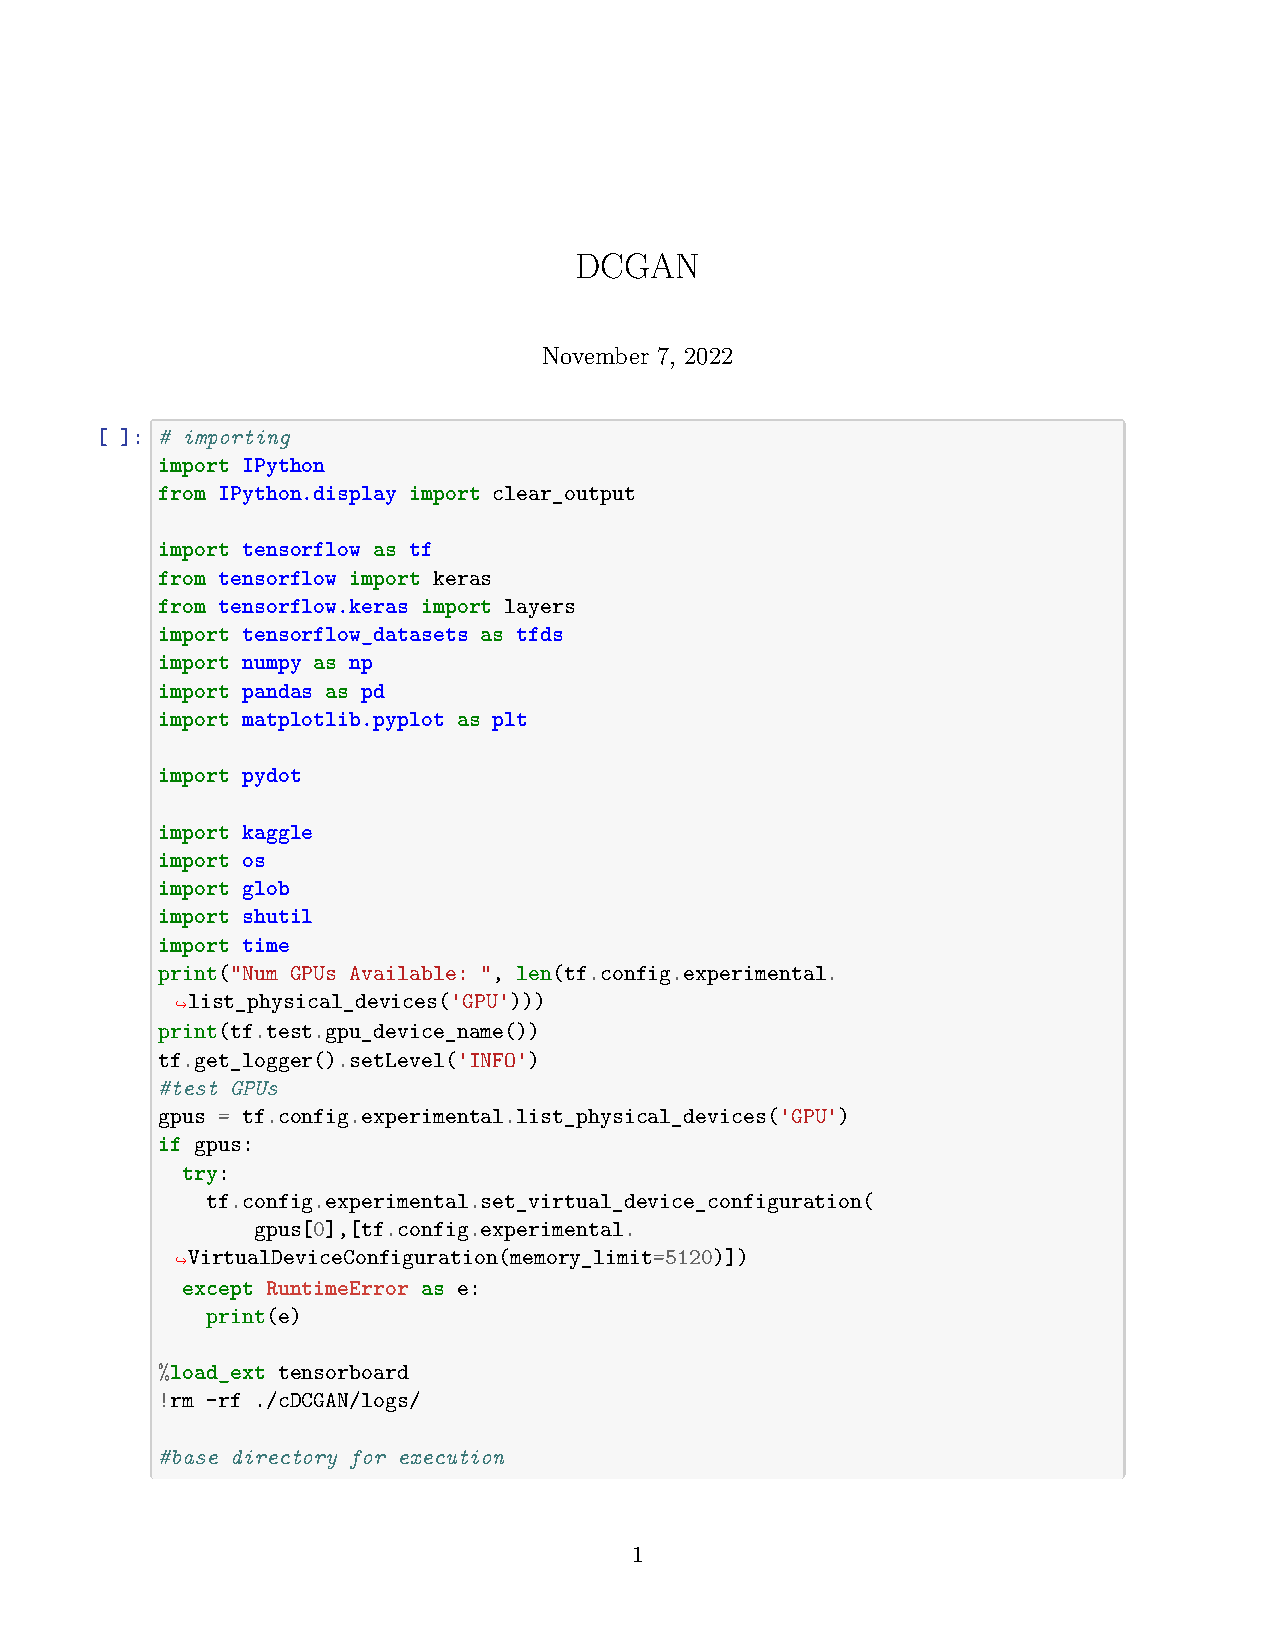
\includepdf[pages=-, addtotoc={1,subsection,2, DCGAN, apx:DCGAN}]{code/DCGAN.pdf}
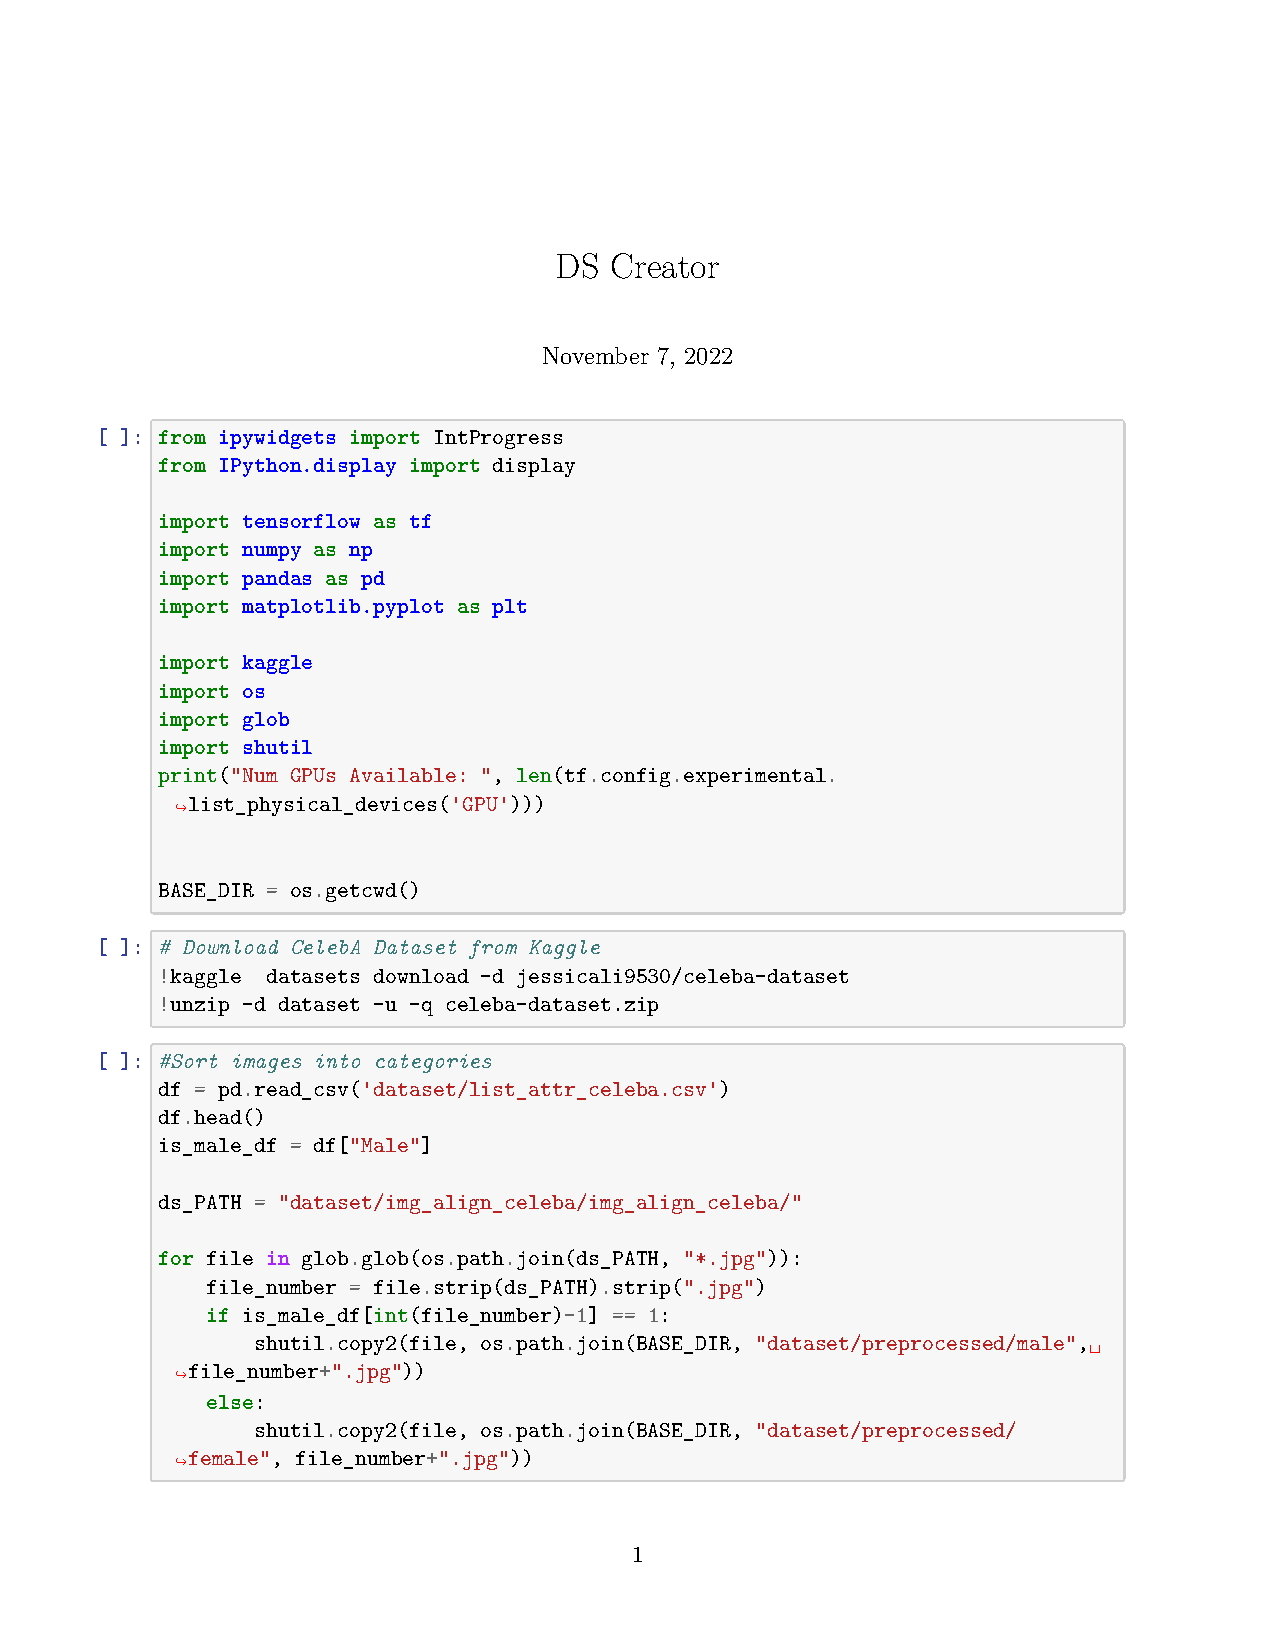
\includepdf[pages=-, addtotoc={1,subsection,2, Dataset Creator, apx:DS_Import}]{code/DSCreator.pdf}
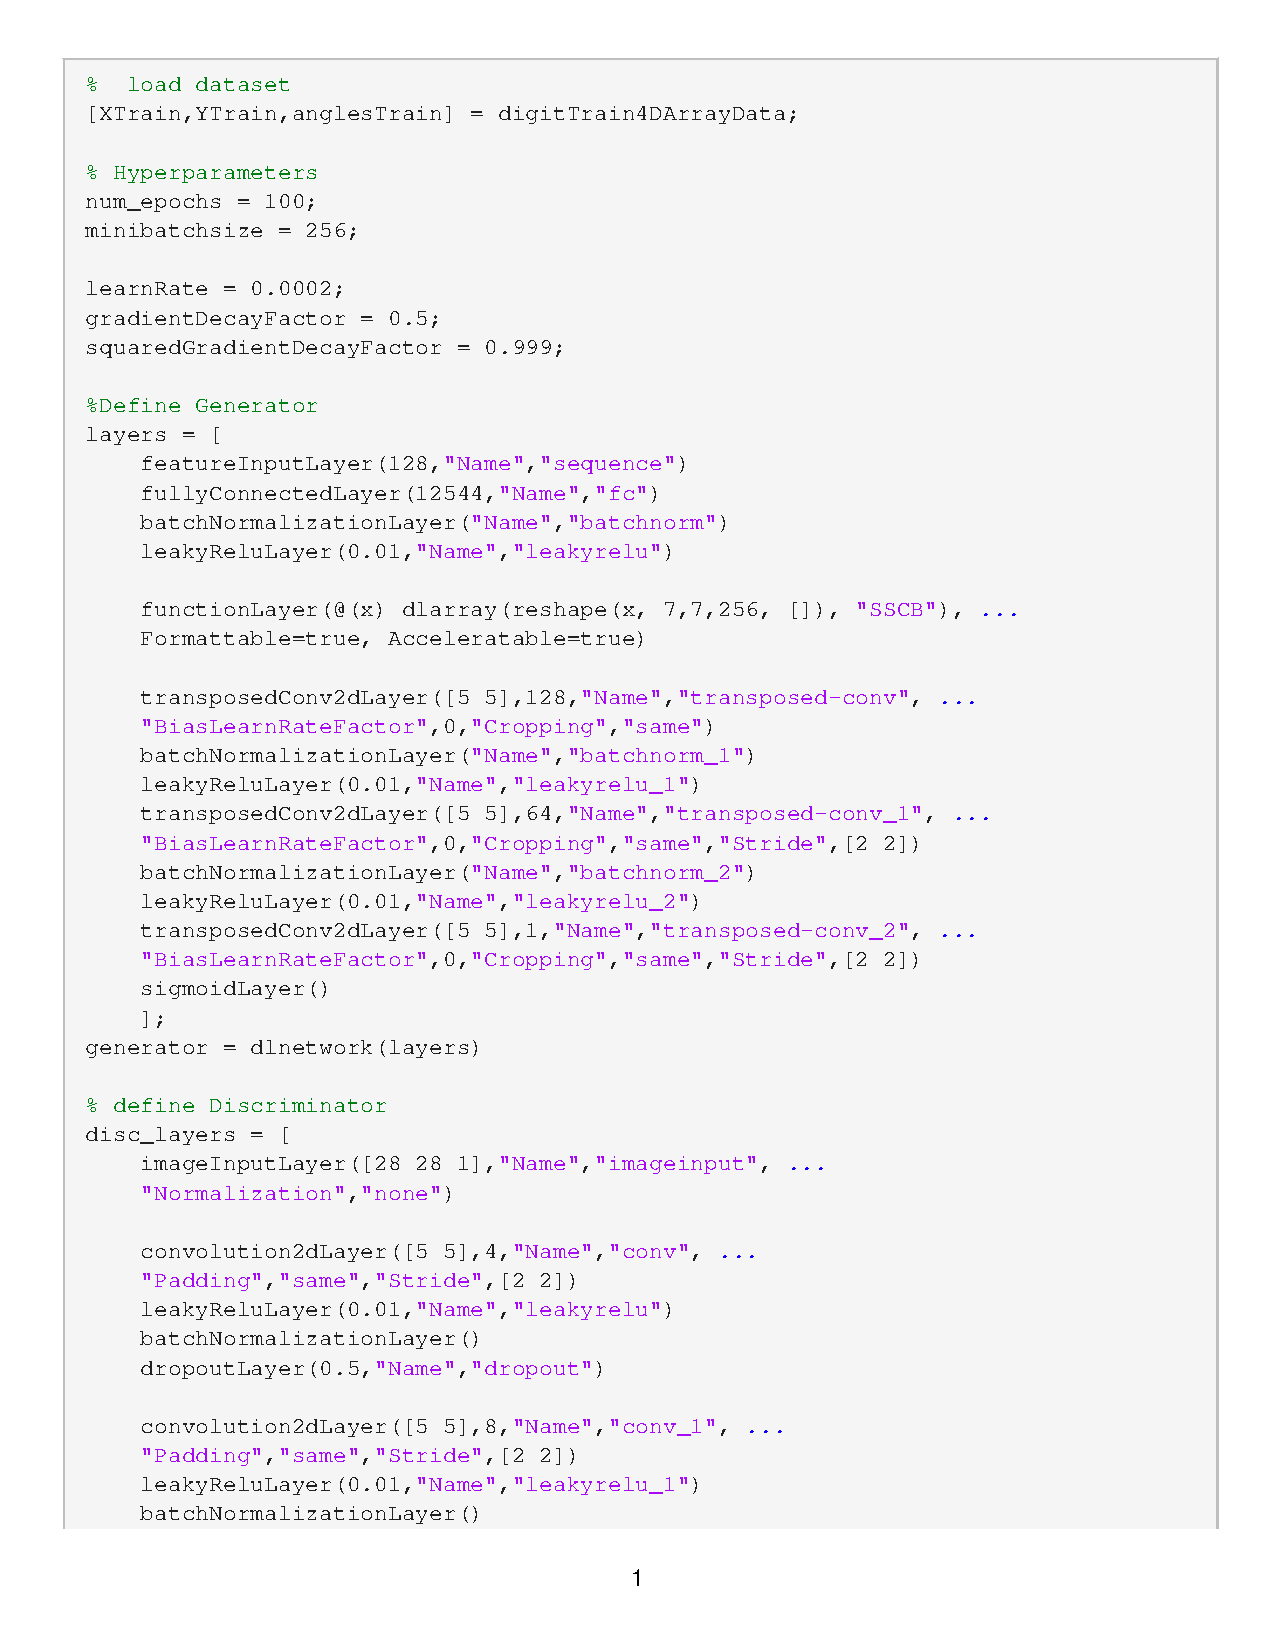
\includepdf[pages=-, addtotoc={1,subsection,2, Matlab GAN, apx:MLGAN}]{code/GAN.pdf}
\end{appendix}

\end{document}
